\chapter{Параллельный алгоритм построения карты проходимости пространства на основе комплексирования разнородных данных}\label{ch:ch4}

В главе~\cref{ch:ch3} описан программный комплекс, реализующий построение карты проходимости пространства на основе множества показаний с датчиков, установленных на БТС. Несмотря на показанную работоспособность для реальных БТС, данный комплекс может задерживать добавление сформированных фрагментов на карту в случае большого количества учитываемых в модели источников данных. Данное свойство комплекса ограничивает число датчиков, которые могут участвовать в уточнении карты проходимости пространства, и, следовательно, ограничивает надёжность строящейся карты.

В данной главе предложены модификации алгоритма построения карты проходимости пространства, реализованного в программном комплексе из главы~\cref{ch:ch3}, позволяющие снизить время обработки информации об окружающем пространстве при добавлении её на карту проходимости пространства, а также избавиться от необходимости последовательного добавления фрагментов на карту, что позволяет увеличить количество комплексируемых источников данных с сохранением возможности работы в режиме реального времени.

\section{Производительность алгоритма построения карты проходимости пространства}\label{sec:ch4/perf}

Представленный в главе~\cref{ch:ch3} алгоритм построения карты проходимости пространства можно разделить на два этапа:

\begin{enumerate}
	\item Преобразование входных данных к единому формату представления данных о проходимости пространства. Как правило, это фрагмент карты проходимости, содержащий вероятности занятости клеток, основываясь на последних показаниях данного источника данных.
	\item Комплексирование полученных фрагментов с раннее построенной картой проходимости пространства. Для обратной модели наблюдения этот шаг заключается в простом суммировании полученного фрагмента с соответствующей областью карты.
\end{enumerate}

Первый шаг допускает параллельное выполнение: для построения фрагмента используются данные только одного источника, и синхронизация с другими источниками и подсистемами не требуется. Его вычислительная стоимость определяется сложностью конкретного алгоритма, однако далее в главе предполагается, что эти алгоритмы уже реализованы оптимальным для целевой системы образом, и потому ускорению не подлежат. Второй шаг, напротив, является блокирующим: созданный фрагмент попадает в очередь и включается в карту лишь после всех фрагментов, стоящих перед ним. Задержка возникает даже тогда, когда добавляемые фрагменты не пересекаются и параллельное обновление теоретически возможно, и растёт с числом источников данных, участвующих в формировании карты. 

Покажем это на практике: на рисунке~\cref{fig:perf-omf} представлены результаты профилирования <<evo\_occupancy\_map\_fusion>> при обработке одного и восьми источников данных. В версии с восемью источниками все провайдеры фрагментов были дубликатами провайдера из запуска с одним источником. Следовательно, все провайдеры обрабатывали одни и те же данные, зарегистрированные в один момент времени. Можно видеть, что из-за последовательного добавления фрагментов на карту проходимости пространства задержки обновления карты проходимости доходят до более чем семикратного замедления.  

\begin{figure}[ht]
	\centerfloat{
		\subcaptionbox{Один источник данных. Время обновления карты -- $3,03$~мс.\label{fig:perf-omf-1}}{
			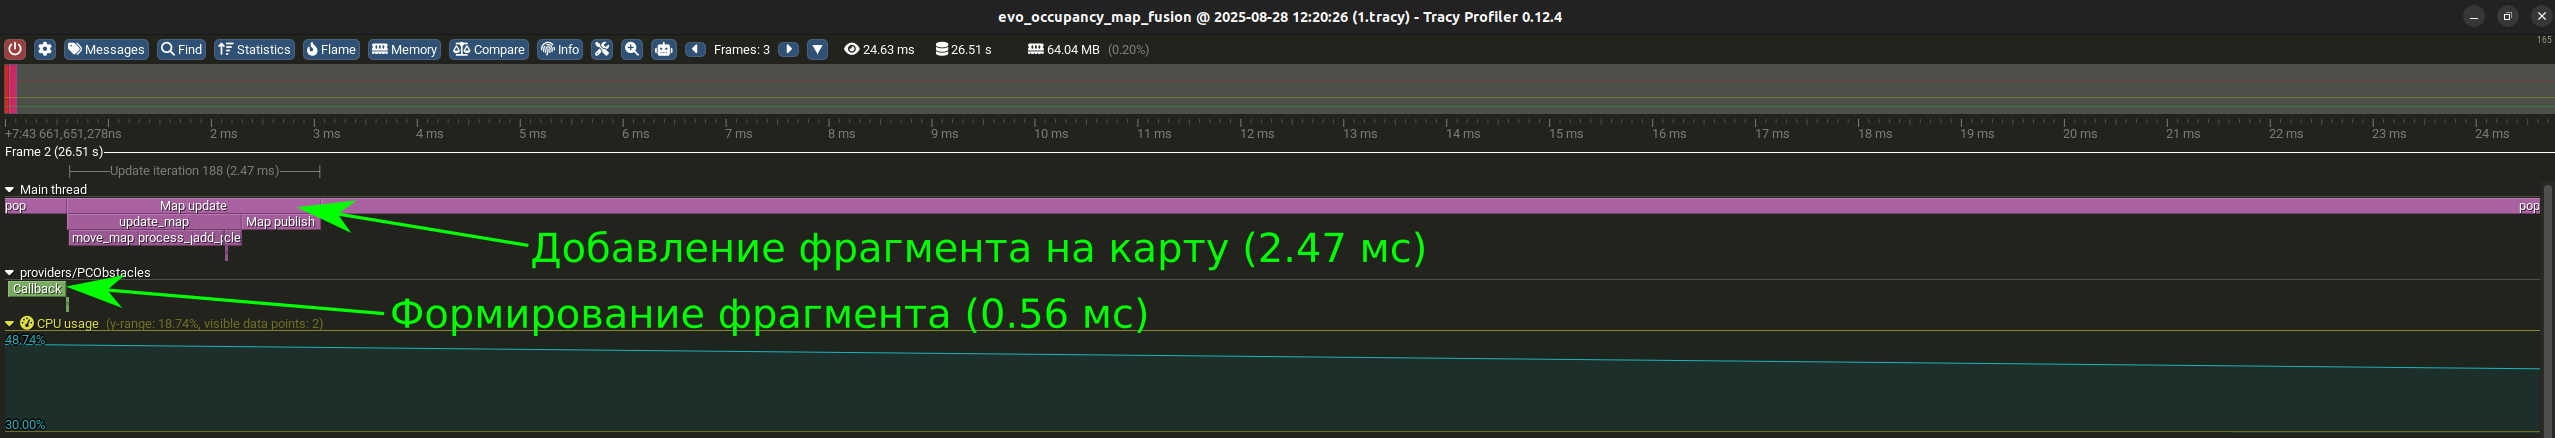
\includegraphics[width=\linewidth]{images/perf-omf-1.png}}\\
		\subcaptionbox{$8$ источников данных. Самое долгое время обновления карты -- $22,78$~мс (замедление на $652$~\%).\label{fig:perf-omf-8}}{
			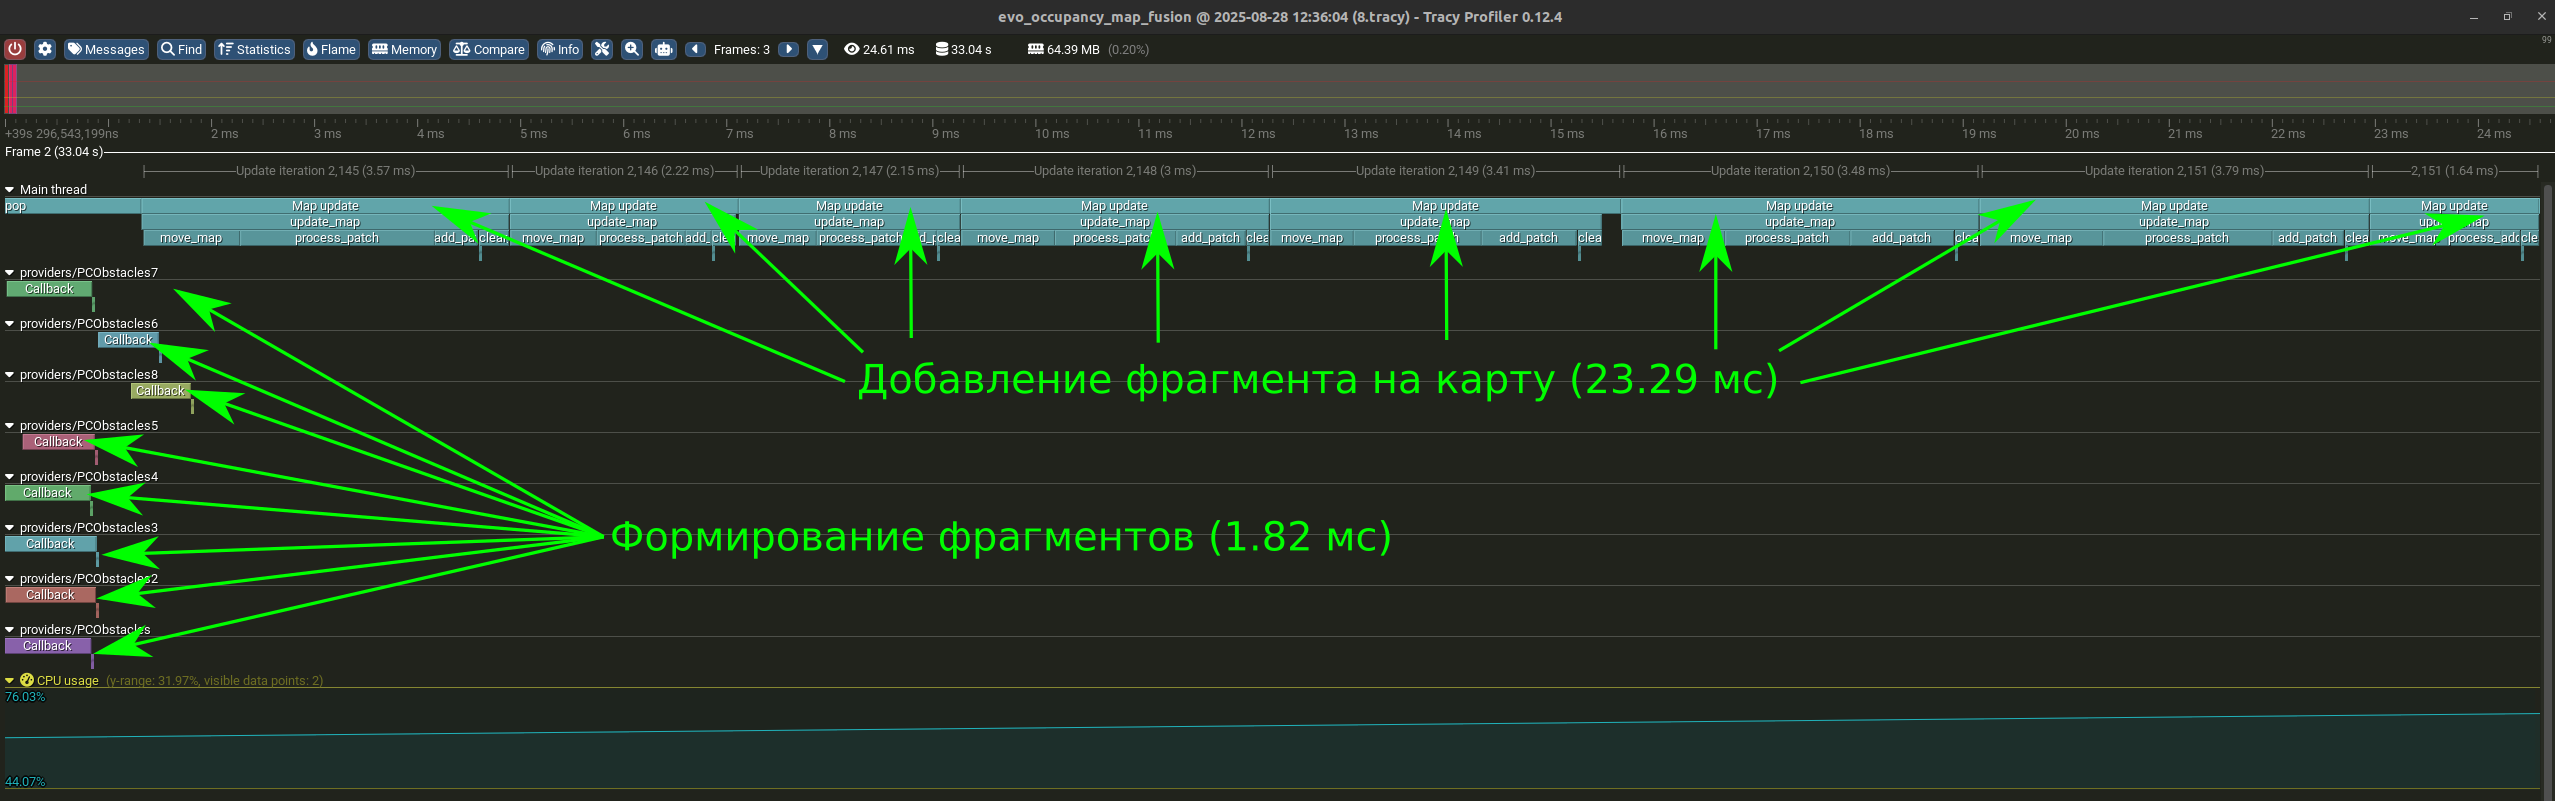
\includegraphics[width=\linewidth]{images/perf-omf-8.png}}\\
	}
	\legend{Результаты профилирования получены в программе инструментального профилирования <<Tracy>>~\cite{kyostila2008tracy}. Приведённые снимки экрана приведены к одному масштабу временной шкалы.}
	\caption{Наблюдаемые задержки при обновлении карты проходимости пространства}\label{fig:perf-omf}
\end{figure}

Далее в главе предложены модификации базового алгоритма построения карты проходимости, направленные на ускорение второго этапа обновления карты проходимости пространства, а также делающие этот шаг асинхронным для каждого источника данных. Перед тем как приступить к описанию модификаций опишем формально задачу, решаемую алгоритмом.

%Проанализируем результаты инструментального профилирования программы реализующей построение карты проходимости пространства. Запуск программы производился на ПК с процессором AMD Ryzen 5 5600x с 6-ю ядрами и тактовой частотой 4.6 ГГц, ОЗУ объёмом 32 Гб, а также ГПУ Nvidia GeForce 3070 с графической памятью 8 Гб и тактовой частотой 1.5 ГГц. Программа обрабатывала данные записанные на реальном БТС в том же формате, в котором они передавались в системе БТС: ROS-сообщениях. Продолжительность профилирования составила $58.7$ секунд. 

%На рисунке предствлен FlameGraph 

% На рисунке~\ref{fig:omf_perf} представлена статистика времени работы отдельных участков главного потока исполнения алгоритма, отвечающего за обновление карты проходимости пространства. 
% \todo[inline, color=red]{тут надо хоть чуть-чуть объяснить что это за данные. Сказать в 2 словах, что мы провели такой0-то эксперимент}
% \todo[inline, color=red]{картикнку я бы преобразовал в гистограмму или круговую диаграмму с абсолютными временами И процентами.}
% Из него видно, что время ожидания доступа к очереди с фрагментами в среднем превышает время непосредственно извлечения фрагмента из очереди, а достигает максимального значения в $~30\%$ от средней продолжительности "полезной" нагрузки -- этапа обновления содержимого карты проходимости пространства. 
% \todo[inline, color=red]{оооочень сложно предложение.Надо разбить на несколько более простых}
% \todo[inline, color=red]{еще было бы хорошо, какой-то простенький расчет тут привести. ЧТо например при таком-то кол-ве сенсоров, задержка уже стоставит столько-то, что означает, что при скорости такой-то уже невозможно будет двигаться. Ну или что-то в таком духе. Ты как ктн должен очень хорошо анализировать практический аспект проблемы, которую решаешь}

% \begin{figure}[!ht]
	%     \centering
	%     \includegraphics[width=\textwidth]{images/omf-perf.png}
	%     \caption{Performance staticstics of a real occupancy grid map algorithm obtained with easy-profiler tool. 'Pop' is a step for a map's patch extraction. This step is divided in two substeps: acquiring mutex lock to access queue ('Wait for lock') and extraction of patch under lock ('Under lock'). 'Map update' is a step for OGM updating: its' content or position, 'Patch processing' substep responsible for the map's content update with an actual vehicle's pose and the obtained patch.}
	%     \label{fig:omf_perf}
	% \end{figure}
%\todo[inline, color=green]{Тут были комментарии про круговые диаграммы, и оценку задержки от числа сенсоров.}

%Целью данной работы является предложить ассинхронный алгоритм построения карты проходимости пространства, который позволяет снизить итоговое время задержки обновления карты.

%Основной вклад данной работы заключается в следующем:
%\begin{enumerate}
%	\item Предложены три последовательные модификации базового алгоритма картирования на основе Байесовского вывода с использованием обратной модели измерения для случая одномерного пространства.
%	\item Проведено сравнение вычислительной сложности базовой реализации и модификаций для всех выполняемых операций над картой проходимости пространства (и их комбинации) при различных размерах картируемой области. Доказано, что применение всех трёх модификаций имеет лучшую вычислителную сложность, чем базовая реализация. %\todo[color=green]{Больше результатов сравнения здесь}
	% \item Предложено расширение итоговой реализации на случай пространства размерности два.
	% \todo[inline, color=red]{до третьего буллета нигде про одномерный случай не говориться, поэтому он выглядит странно. Его надо либо убрать, либо где-то ране упомянуть одномерный случай. Я скорее за первый подход (убрать) в статье и за второй в диссере.}
%\end{enumerate}

%Далее глава организована следующим образом: в разделе~\ref{sec:map_description} мы формулируем постановку задачи построения карты проходимости, описываем операции производимые над ней и описываем их базовую реализацию. В следующем разделе~\ref{sec:implementations} мы предлагаем модификации базовой реализации, позволяющие уменьшить вычислительную сложность операций, для упрощения восприятия в данном разделе мы упростим задачу и будем рассматривать карту, как одномерное пространство. Далее в разделе~\ref{sec:experiments} представлены эксперименты со сравнением вычислительной сложности всех представленных модификаций и исходной реализации для каждой операции в отдельности и их комбинации. В разделе~\ref{sec:2D_implementation} мы приводим обобщение последней модификации, показавшей лучшую вычислительную сложность, на случай двумерного пространства. В последнем разделе~\ref{sec:conclusion} проводится анализ полученных результатов.

\section{Постановка задачи построения карты проходимости пространства}\label{sec:map_description}

Зафиксируем неподвижную относительно земли глобальную систему координат, расположенную так, что движение БТС происходит в плоскости $z = 0$. Положение БТС в ней описывается тройкой $\textbf{x} = x, y, \theta$: координатами $x, y$ фиксированной точки БТС и углом $\theta$ поворота БТС от оси $Ox$ вокруг вертикальной оси (рисунок~\ref{fig:map_coords}). С той же фиксированной точкой свяжем локальную систему координат БТС, ось $Ox$ которой направлена вдоль оси его движения; координаты в ней обозначаются $x_l, y_l$.

Пусть на БТС имеется $S$ источников данных, каждый со своей системой координат, положение которой известно и неизменно относительно локальной. Независимо от остальных источник $s$ порождает сведения о занятом и\slash или свободном пространстве в окрестности БТС в виде наборов $(P_{s,k}, \textbf{x}_{s,k}, t_{s,k})$, $s=\overline{1,S}$, $k\in\mathbb{N}$. Здесь $P_{s,k}$ -- фрагмент карты проходимости, то есть двумерный массив логарифмов шансов занятости пространства с фиксированным разрешением $res_s$ (pixel per meter, элементов на метр), оси которого ориентированы вдоль осей системы координат источника $s$; $\textbf{x}_{s,k}$ задаёт положение начала системы координат датчика относительно левого верхнего угла массива; $t_{s,k}$ -- время регистрации данных, по которым построен фрагмент; $k$ -- порядковый индекс набора. 

По этим данным требуется сформировать локальную карту проходимости пространства в виде набора $(M_i, \textbf{x}_i, t_i)$, $i\in\mathbb{N}$, где $M_i$ -- двумерный массив логарифмов шансов занятости пространства с фиксированным разрешением $res$, соответствующий моменту времени $t_i$, а $\textbf{x}_i$ -- координаты левого верхнего угла карты. Координаты $\textbf{x}_i$ выбираются так, чтобы начало локальной системы координат в момент $t_i$ приходилось на центр карты $M_i$, при этом оси карты остаются параллельными осям глобальной системы координат. Такая ориентация выбрана не случайно: при ориентации карты вдоль осей локальной системы координат каждое изменение курса БТС требовало бы поворота двумерного массива на малый угол, и накопление подобных поворотов вносило бы погрешность в оценку положения свободного и занятого пространства.

\begin{figure}[ht!]
	\centering
	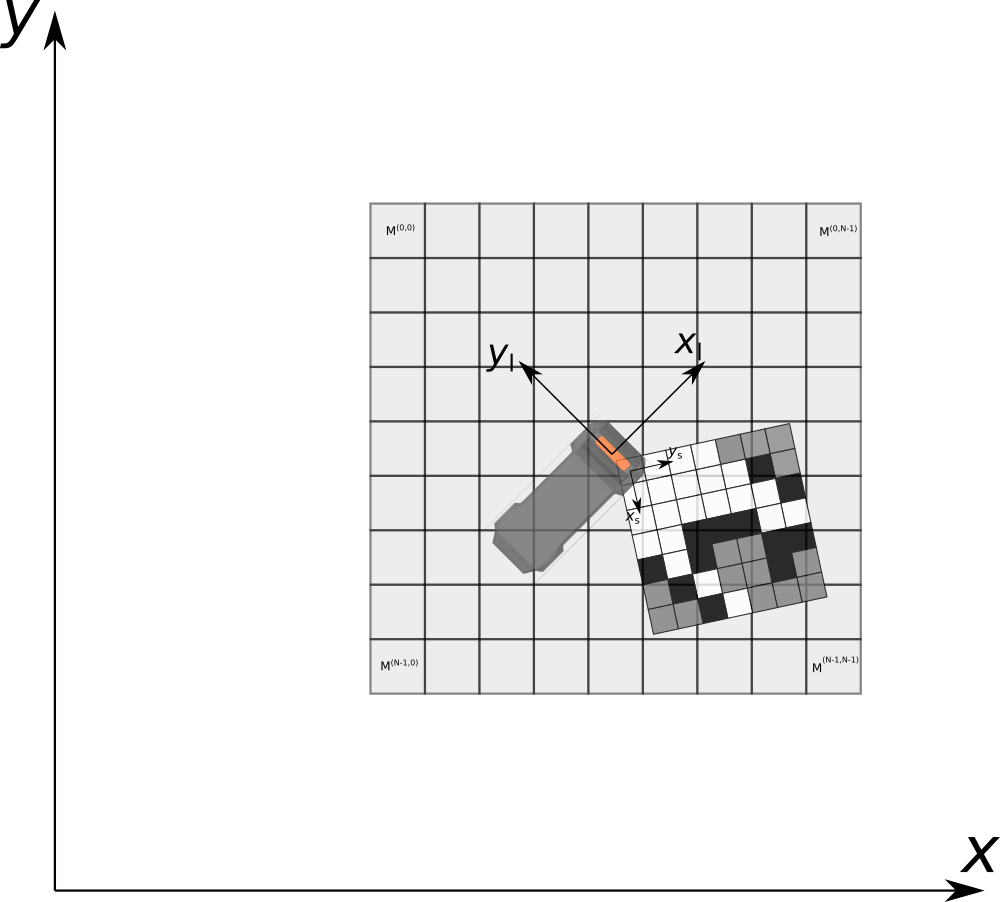
\includegraphics[width=0.7\textwidth]{images/map_coords.png}
	\caption{Расположение локальной карты проходимости и её фрагмента от одного из источников данных  относительно БТС и глобальной системы координат.}
	\label{fig:map_coords}
\end{figure}


Генерируемые фрагменты $P_{s,k}$ поступают в общую очередь по мере готовности, а локальная карта обновляется последовательным извлечением фрагментов из этой очереди. Порядок извлечения определяется моментом готовности фрагмента, а не моментом регистрации данных, поэтому последовательность времён $t_{s,k}$ в общем случае не монотонна (рисунок~\ref{fig:patch_order}).

Одна итерация обновления приведена в листинге~\ref{code:update} и состоит из трёх действий. Во-первых, если извлечённый фрагмент новее карты, карта актуализируется: её положение и время заменяются положением БТС и временем регистрации фрагмента, а содержимое сдвигается и экспоненциально затухает (назначение затухания описано далее в этом разделе). Во-вторых, фрагмент приводится к системе координат карты: <<доворачивается>> до её ориентации, масштабируется до её разрешения, и вычисляется смещение $patch\_shift$ его левого верхнего угла относительно угла карты; если фрагмент старше карты, затухание применяется к нему, а не к ней. В-третьих, преобразованный фрагмент поэлементно суммируется с соответствующей ему областью карты (рисунок~\ref{fig:update_demo}).

\begin{figure}[ht!]
	\centering
	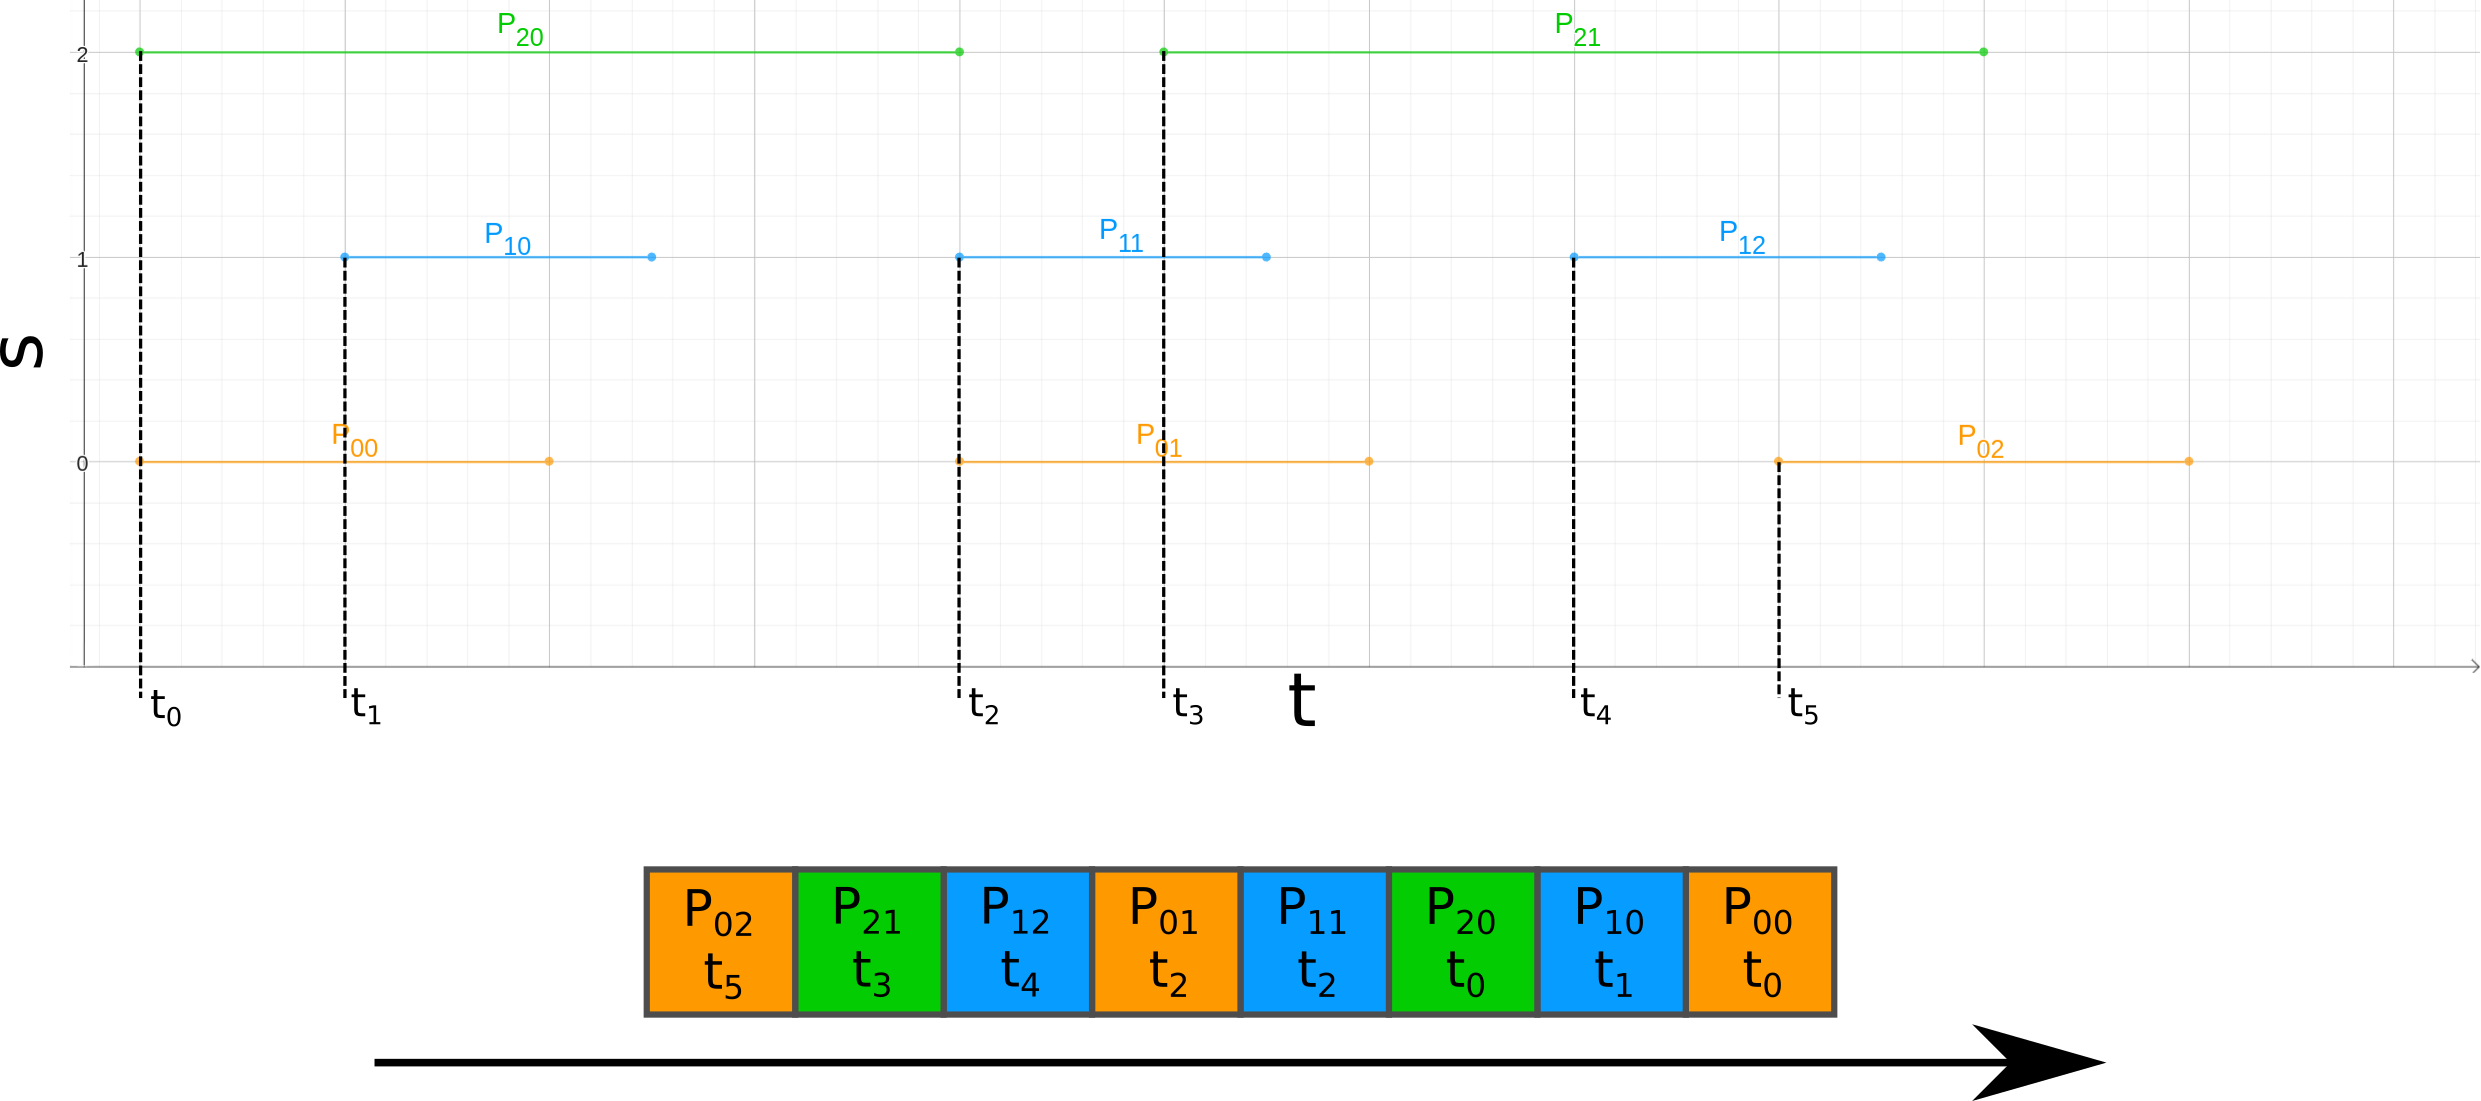
\includegraphics[width=\textwidth]{images/PatchOrder.png}
	\caption{Демонстрация формирования очереди фрагментов. Горизонтальные отрезки обозначают время формирования фрагмента каждым источником: начало отрезка соответствует времени регистрации данных $t_{s,k}$, конец отрезка соответствует времени завершения формирования фрагмента и моменту добавления его в очередь фрагментов. Внизу иллюстрации продемонстрирован итоговый порядок фрагментов в очереди: фрагменты извлекаются из очереди в порядке справа налево.}
	\label{fig:patch_order}
\end{figure}

\begin{algorithm}
	\LinesNumbered
	\caption{Добавление фрагмента на карту: $update\_map$.}
	\label{code:update}
	\KwIn {$P_{s,k}$ -- фрагмент извлечённый из очереди;\\ 
		   $x_{s,k}$ -- положение извлечённого фрагмента;\\
		   $t_{s,k}$ -- время регистрации извлечённого фрагмента;\\ 
		   $x_{i-1}, t_{i-1}$ -- положение БТС и время при последнем обновлении карты;\\
		   $M_{i-1}$ -- карта проходимости пространства после последнего обновления;\\
		   $res$ -- разрешение карты проходимости;\\
		   $res_s$ -- разрешение извлечённого фрагмента;
		  }
    \KwOut {$M_i$ -- карта после добавления фрагмента}
	\eIf{$t_{s,k} > t_{i-1}$}{
		$x_i \gets get\_map\_pose(t_{s,k})$\;
		$t_i \gets t_{s,k}$\;
		$M_{actual} \gets shift\_map(M_{i-1}, x_i - x_{i-1})$\;
		$M_{actual} \gets dim(M_{actual}, t_i - t_{i-1})$\;
    }{
		$x_i \gets x_{i-1}$\;
		$t_i \gets t_{i-1}$\;
		$M_{actual} \gets M_{i-1}$\;
	}
	$P_{aligned}, patch\_shift \gets align\_patch(P_{s,k}, t_{s,k}, t_{i}, res / res_{s})$\;
	$P_{aligned} \gets dim(P_{aligned}, t_i - t_{s,k})$\;
	$M_i \gets add\_patch(M_{actual}, P_{aligned}, patch\_shift)$\;
	\Return {$M_i$}
\end{algorithm}

\begin{figure}[ht!]
	\begin{subfigure}{\textwidth}
		\centering
		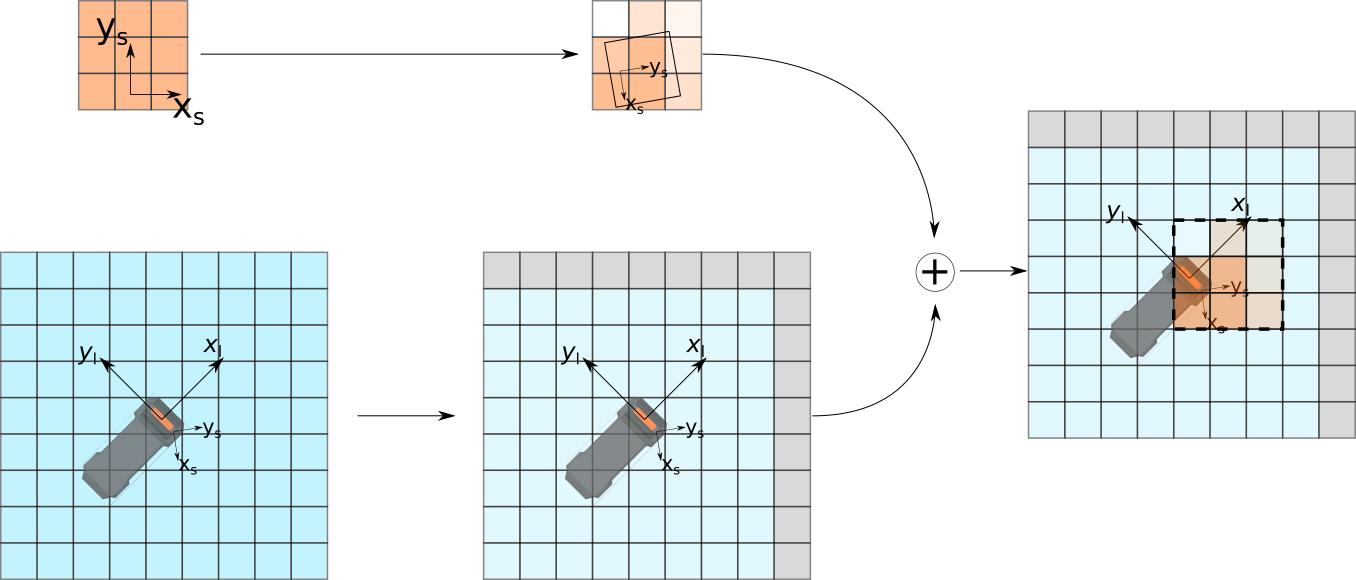
\includegraphics[width=.8\linewidth]{images/old_map.png}
		\caption{Время регистрации фрагмента новее последнего времени обновления карты.}
		\label{subfig:update_demo_old_map}
	\end{subfigure}
	
	\begin{subfigure}{\textwidth}
		\centering
		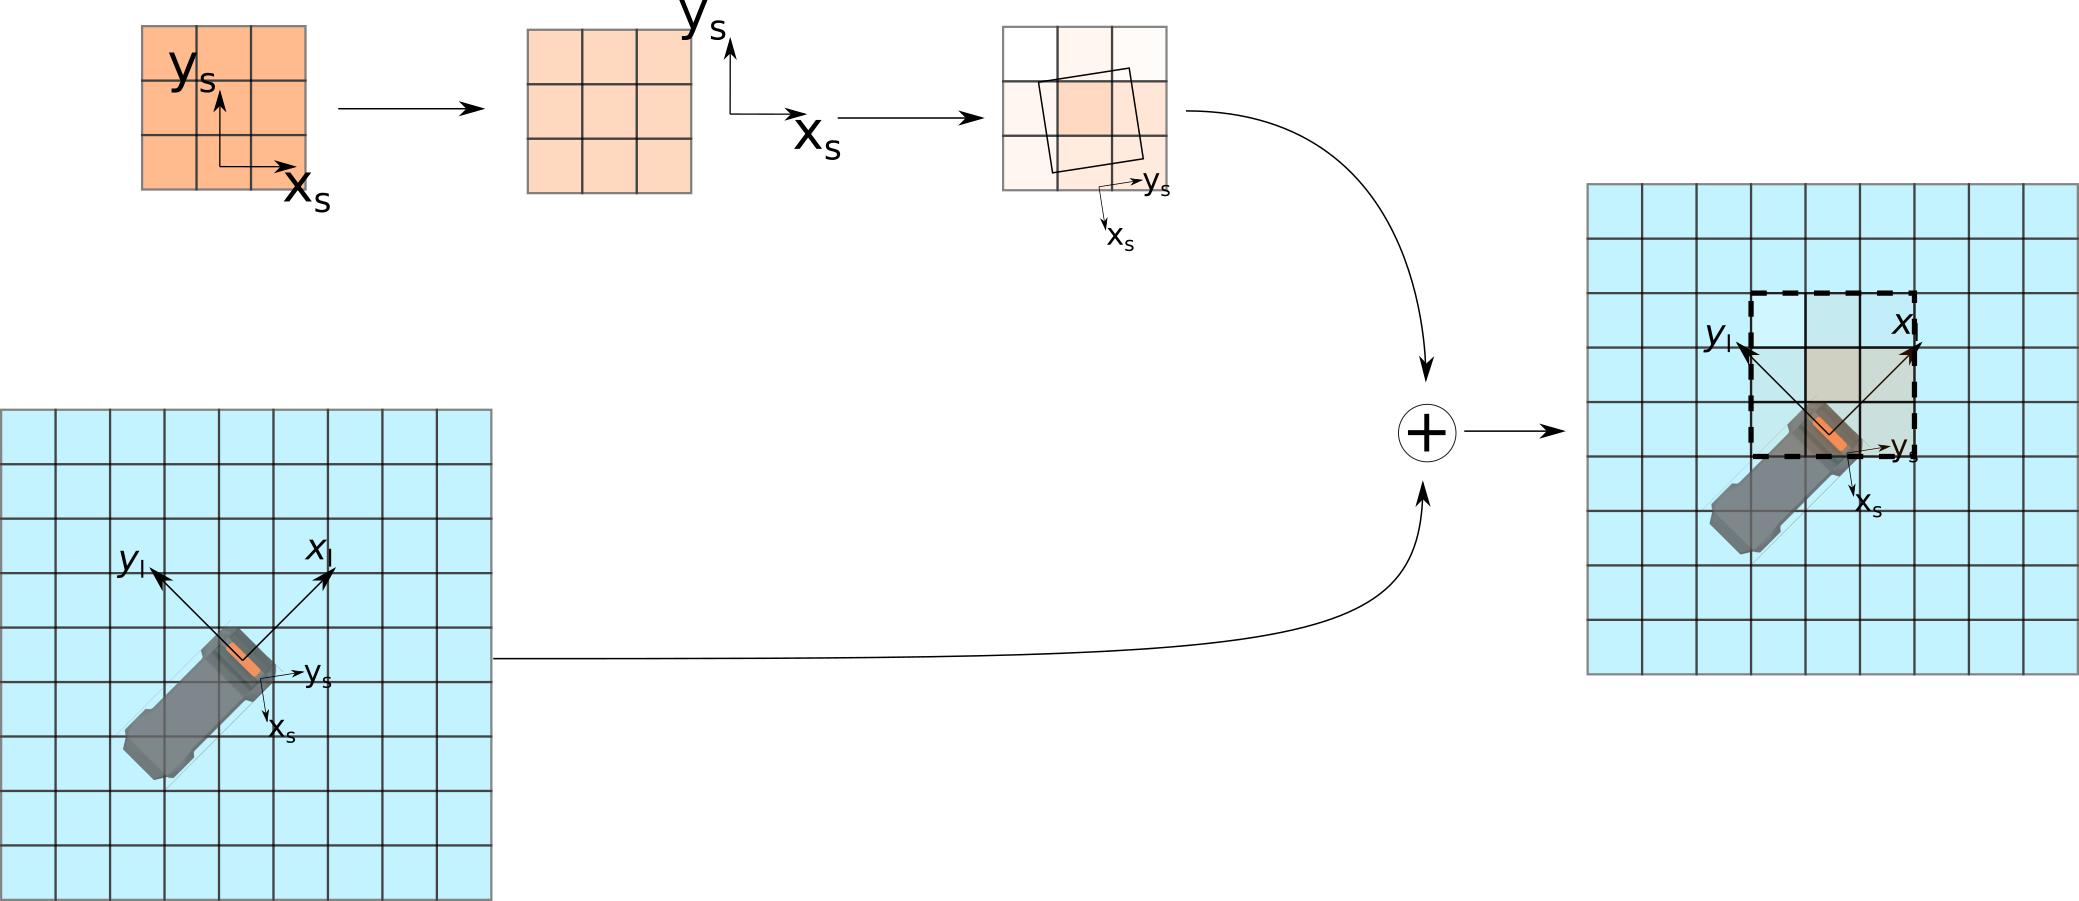
\includegraphics[width=.8\linewidth]{images/old_patch.png}
		\caption{Время регистрации фрагмента старше последнего времени обновления карты.}
		\label{subfig:update_demo_old_patch}
	\end{subfigure}
	\caption{Иллюстрация алгоритма добавления фрагмента от источника данных $s$ на локальную карту проходимости пространства.}
	\label{fig:update_demo}
\end{figure}

Недостатком обратной модели наблюдения является предположение о статичности сцены: в случае наличия динамических объектов в сцене, такие объекты оставляют за собой <<след>>, который не удаляется с локальной карты проходимости пространства, если нет источника данных, способного отмечать области, в которых препятствия отсутствуют. Даже при наличии такого источника, <<след>> может попасть в его слепую зону и остаться на карте. Для решения данной проблемы применяется экспоненциальное затухание значений в клетках карты, постепенно возвращающее их в состояние <<неизвестно>> без повторных обновлений от источников данных. Операция затухания $dim(\widehat{M}, \Delta t)$, применяемая в листинге~\ref{code:update} как к карте, так и к фрагменту, поэлементно пересчитывает их значения:

\begin{equation}
	\widehat{M}_{i}^{\,j,k} = \exp(-a\,\Delta t)\;\widehat{M}_{i-1}^{\,j,k},
	\label{eq:dim}
\end{equation}

где $\Delta t \geq 0$ -- разница между текущим временем и временем регистрации $\widehat{M}$, а $a$ -- гиперпараметр, задающий скорость затухания.

Одного затухания, однако, недостаточно. Долго стоявшее неподвижно динамическое препятствие успевает накопить в занимаемых им клетках большой по модулю логарифм шансов ($|l_t| \gg 0$), и после того как препятствие сдвинулось, освободившееся пространство ещё долго квантуется как занятое: возврат таких клеток в состояние <<неизвестно>> или <<свободно>> за счёт одного лишь затухания занимает продолжительное время. Чтобы исключить такую <<перезарядку>>, на шаге добавления фрагмента абсолютная величина значения клетки ограничивается сверху:

\begin{equation}
	l_{t} = \max\left(\min\left[\text{inv\_obs\_model}(t), l_{thresh}\right], -l_{thresh}\right),
	\label{eq:l_clip}
\end{equation}
где $\text{inv\_obs\_model}(t)$ -- значение логарифма шансов, полученное по формуле~\cref{eq:log_odd_upd}, $l_{thresh}$ -- пороговое значение логарифма шансов по абсолютному значению.

\section{Модификации базовой реализации}\label{sec:implementations}

В данном разделе предлагаются модификации базовой реализации для снижения задержки между появлением информации о проходимости у одного из источников данных и её добавлением на итоговую карту проходимости пространства. Чтобы упростить изложение, пространство далее считается одномерным: карта в таком случае представляет собой одномерный массив $M$ размера $N$, а движение возможно только влево или вправо. Размер одной клетки также принимается равным $1$ метру, чтобы опустить операции с учётом разрешения карты $res$. В предыдущем разделе показано, что карта должна поддерживать операции сдвига и добавления фрагмента. Помимо них к описанию реализаций отдельно добавлена операция получения карты, поскольку в модификациях данная операция перестаёт быть тривиальным копированием массива и требует отдельного обсуждения.  

\subsection{Базовая реализация}

Опишем исходную реализацию в одномерном случае. Карта представляет собой массив $M$ размера $N$, текущую координату центра $x_i$ и время $t_i$, которому это состояние карты соответствует (рисунок~\ref{fig:base_omf}).

\begin{figure}[!ht]
	\centering
	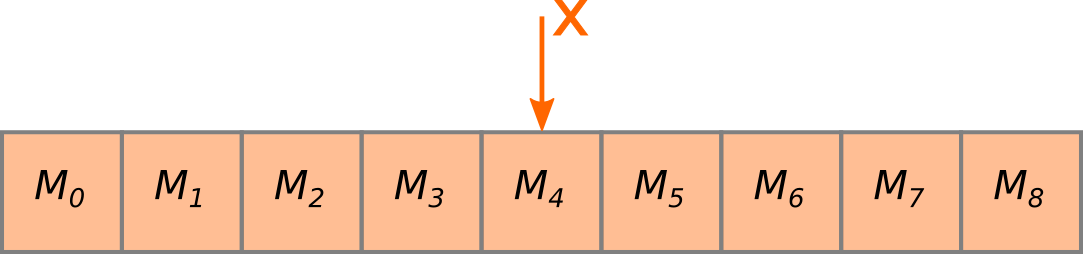
\includegraphics[width=\textwidth]{images/BaseOMF.png}
	\caption{Оригинальная реализация локальной карты проходимости пространства.}
	\label{fig:base_omf}
\end{figure}

\textbf{Сдвиг.} При переходе в новую точку $x_{i+1}$ в момент времени $t_{i+1}$ массив со значениями логарифма шансов проходимости сдвигается на $\lfloor x_{i+1} - x_{i}\rceil$ клеток, а клетки, для которых прежних значений не существует, инициализируются нулём. Операция затрагивает весь массив, поэтому её вычислительная сложность $\Theta(N)$.

\textbf{Добавление фрагмента.} Операция повторяет листинг~\ref{code:update} с двумя упрощениями, следующими из одномерности задачи: <<доворачивание>> фрагмента не требуется, а из преобразований его координат остаётся лишь учёт сдвига карты за промежуток между моментом регистрации фрагмента и итоговым временем карты. Далее размер фрагмента $P$ обозначается $N_P$.

Часть операции, предшествующая поэлементному суммированию, имеет сложность $\Theta(1)$, если $t_{s,k} \le t_{i-1}$, и $\Theta(N)$ в противном случае, поскольку требует сдвига и затухания всей карты. Само суммирование выполняет $\Theta(N_P)$ операций, если фрагмент целиком помещается на карту, $\Theta(N)$ операций, если фрагмент больше карты и полностью её покрывает, и не выполняется вовсе, если фрагмент с картой не пересекается. Тем самым сложность суммирования составляет $O(\min(N_P, N))$, а всей операции --- $O(N + \min(N_P, N))$.

\textbf{Получение карты.} Возвращается копия текущего массива, что требует $\Theta(N)$ операций. Копия необходима, чтобы на время передачи карты потребителям не блокировать последующие операции сдвига и добавления фрагментов.

\subsection{Расширенная карта проходимости пространства}

Первая модификация локальной карты проходимости пространства направлена на снижение стоимости сдвига. Массив для хранения карты увеличивается до размера $\widehat{N} > N$, чтобы описывать область больше отображаемой, а к координате $x$ отображаемой части добавляется координата $\widehat{x}$ некоторой фиксированной точки <<полного>> массива; в качестве такой точки возьмём его центр (рисунок~\ref{fig:prefetched_omf}).

\begin{figure}[!ht]
	\centering
	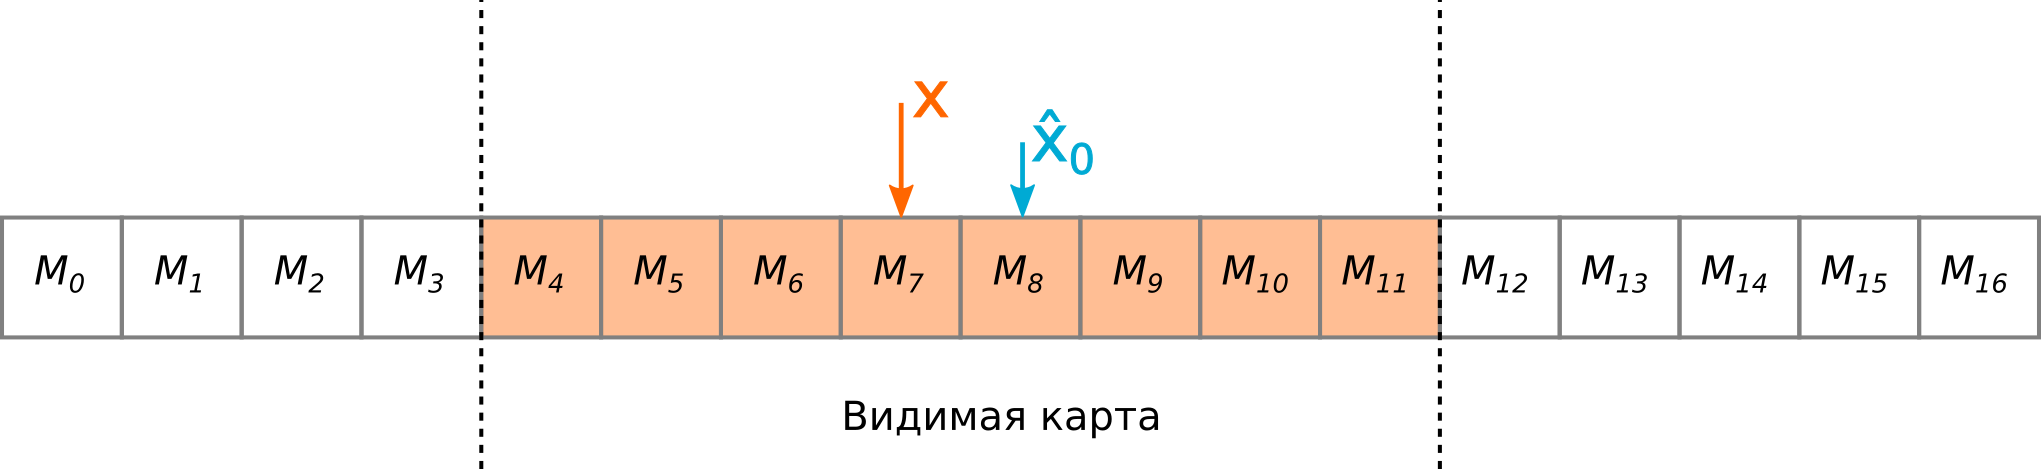
\includegraphics[width=\textwidth]{images/PrefetchedOMF.png}
	\caption{Карта с предподготовленными окрестностями.}
	\label{fig:prefetched_omf}
\end{figure}

\textbf{Сдвиг} в общем случае сводится к обновлению значения $x$ и потому требует $\Theta(1)$ операций. Содержимое массива сдвигается, как в базовой реализации, только когда отображаемая часть карты выходит за границы полного массива, то есть когда $\widehat{x} - x_{i+1} \notin [N/2;\, \widehat{N} - N/2)$; тогда содержимое сдвигается так, чтобы новый $\widehat{x}$ совпал с актуальным $x$, что стоит $\Theta(\widehat{N})$ операций. При правильно выбранном размере массива амортизированная сложность операции составляет $\Theta(1)$.

\textbf{Добавление фрагмента} в точности повторяет одноимённую операцию базовой реализации. Её сложность --- $O(\min(N_P, N))$, если затухание карты не выполняется, и $O(\widehat{N} + \min(N_P, N))$ в противном случае: затуханию подлежат и клетки за границами видимой области, поскольку они могли быть обновлены ранее и вернуться в неё при последующих сдвигах.

\textbf{Получение карты} заключается в копировании подмассива, соответствующего видимой части карты, и требует, как и прежде, $O(N)$ операций. Все операции по-прежнему остаются блокирующими.

\subsection{Карта с разделяемыми блокировками}

С ростом числа источников данных узким местом алгоритма становятся блокировки: источник ждёт своей очереди на доступ к карте даже тогда, когда добавляемые фрагменты между собой не пересекаются. Вторая модификация снижает эту задержку, изменяя структуру самой клетки карты. Вместо одного числа с плавающей точкой клетка хранит атомарную пару <<значение логарифма шансов занятости -- время, которому это значение соответствует>>. Требование, чтобы все клетки массива относятся к одному моменту времени, тем самым снимается. Размер атомарной структуры данных, то есть структуры, не использующей при чтении и записи примитивы блокировки (мьютексы, семафоры, сигналы и т.п.), должен быть согласован с возможностями аппаратного обеспечения. Здесь структура состоит из двух 32-битных полей, то есть занимает 64 бита, а атомарные операции с данными такого размера поддерживаются инструкциями большинства современных архитектур~\cite{fog2014lists}.

\textbf{Сдвиг} не претерпел значительных изменений в сравнении с предыдущей реализацией: при копировании клеток во время <<полноценного>> сдвига копируется не только значение логарифма шансов, но и время, а новые клетки требуют инициализации времени (используется значение $0$, поскольку оно не влияет на последующие обновления клетки). Сложность операции остаётся амортизированной $\Theta(1)$ и $\Theta(\widehat{N})$ в худшем случае, однако реальная константа увеличивается: копирование и инициализация атомарных структур заметно продолжительнее, чем у неатомарных аналогов.

\textbf{Добавление фрагмента} во многом повторяет одноимённую операцию предыдущей реализации. Сначала проверяется, требуется ли сдвиг карты. Если не требуется, операция выполняется одновременно с другими такими же операциями; если требуется, она дожидается исключительных прав на модификацию карты и производит сдвиг.

Затем корректируются координаты области, в которую добавляется фрагмент, и обновляются её клетки. Значение очередной клетки считывается атомарно, по нему с учётом затухания вычисляется новое значение (формула~\cref{eq:dim}), и результат записывается обратно операцией сравнения с обменом (Compare and Swap, CAS) -- то есть только при условии, что за время вычисления значение клетки не изменилось. Если условие не выполнено, новое значение пересчитывается уже от обновившегося состояния клетки, и попытка повторяется до успешной записи. Описанный алгоритм приведён в листинге~\ref{alg:partially_lockfree_upd}.

\begin{algorithm}
	\small
	\caption{Добавление фрагмента (модификация с  разделяемыми блокировками): $update\_map(P_s, t_{s,k}, x_{s,k})$.}\label{alg:partially_lockfree_upd}
	\KwIn{$M$ -- карта проходимости пространства;\\ 
		$P_s$ -- добавляемый фрагмент;\\ 
		$x_{t_{s,k}}$ -- положение карты $M$ в момент $t_{s,k}$;\\
		$x_{s,k}$ -- положение источника данных $s$ в момент регистрации фрагмента;}
	\KwOut {$M$ после добавления фрагмента}
	\tcp{Область с возможностью одновременного добавления фрагментов}
	$shared\_lock(map\_access\_mutex)$\;
	$x_{t_{s,k}} \gets \text{local occupancy map pose at } t_{s,k}$\;
	\eIf{\text(Нужен сдвиг $M$)}{
		\tcp{Начало критической секции}
		$unique\_lock(map\_access\_mutex)$\;
		\eIf{Сдвиг по-прежнему нужен и не произошёл в другом потоке до входа в критическую секцию}{
			$M \gets shift\_map(M, x_{t_{s,k}})$
		}{
			$x_{s,k} \gets x_{s,k} - (x_{t_i} - x_{t_{s,k}})$\;
		}
		\tcp{Конец критической секции}
	}{
	  $x_{s,k} \gets x_{s,k} - (x_{t_i} - x_{t_{s,k}})$\;
	}
	$\Delta x_{s} \gets \text{round}(x_{s,k} - x_{i})$\;
	\For {$j \gets \max(0, \Delta x_{s})$ \KwTo $\min(N_P;N + \Delta x_{s})$}{
		$t_{prev} \gets 0$\;
		$val_{prev} \gets 0$\;
		$t_{new} \gets t_{s,k}$\;
		$val_{new} \gets P_s[j]$\;
		\BlankLine
		\While {При $CAS(M[j - \Delta x_{s}], \{val_{prev}, t_{prev}\}, \{val_{new}, t_{new}\})$ обмен не произошёл}{
			\tcp{Значение $\{val_{prev}, t_{prev}\}$ актуализируются в случае неудачной операции сравнения с обменом}
			\eIf{$t_{prev} < t_{s,k}$}{
				$t_{new}  \gets t_{s,k}$\;
				$val_{new}  \gets val_{prev} \exp(-a(t_{s,k} - t_{prev})) + P_s[j]$\;
			}{
				$t_{new}  \gets t_{prev}$\;
				$val_{new}  \gets val_{prev} + P_s[j] \exp(-a(t_{prev} - t_{s,k}))$\;
			}
		}
	}
\end{algorithm} 

Теоретически данная операция может выполняться неограниченно долго, если между попытками сравнения с обменом происходит обновление значения клетки в другой операции. На практике незавершаемость операции практически невозможна ввиду в первую очередь ограниченного числа потоков, работающих одновременно (в рассматриваемом случае их $12$, на современных вычислителях, используемых в робототехнике их число варьируется от $8$ до $24$). Если пренебречь единичными перерасчётами обновляемых значений, сложность такой операции становится $O(\min(N_P, N))$ ($O(\widehat{N} + \min(N_P, N))$, если во время выполнения операции произошёл <<полноценный>> сдвиг карты). Однако константа в этом случае будет заметно больше, чем в предыдущих вариантах из-за использования а) атомарных операций, которые в несколько раз вычислительно дороже неатомарных аналогов и б) shared\_mutex, который имеет значительно большее время блокировки в сравнении с обычным mutex-ом. Поэтому эта реализация становится выгоднее предыдущих вариантов при условии достаточного количества источников, производящих одновременное добавление фрагментов на карту. 

\textbf{Получение карты.} Чтобы исключить состояние гонки с другими операциями, клетки видимой части карты копируются целиком, и одновременно среди них отыскивается наиболее позднее время $t_{newest}$. По копии строится карта <<старого>> формата -- массив чисел с плавающей точкой, значения которого приведены к моменту $t_{newest}$. Сложность операции $O(N)$, но, как и при добавлении фрагмента, скрытая за $O$ константа превышает прежнюю. Эта операция допускает одновременное выполнение с добавлением фрагментов, если частично обновлённое состояние карты приемлемо. Рассмотрим, например, такой сценарий:

\begin{enumerate}
	\item Операция получения карты считала значение $M[0]$
	\item Источник данных обновил значения клеток $M[0]$, $M[1]$
	\item Операция получения карты считала значение $M[1]$
\end{enumerate}

В этом случае только в $M[1]$ будут учтены показания источника данных. Естественно, в последующих вызовах эти показания будут учтены в обеих клетках. Если такая несогласованность данных считается недопустимой, операция получения карты должна быть блокирующей аналогично сдвигу.

\subsection{Карта проходимости пространства с полным обновлением без блокировок}

Последняя модификация снимает оставшееся ограничение и делает неблокирующей также операцию сдвига. Карта разбивается на два равных примыкающих друг к другу фрагмента размера $\widehat{N}$ каждый; к фрагменту добавляется координата его положения (как и ранее -- центр), а сами фрагменты хранятся в разделяемых умных указателях $pM_{1}, pM_{2}$ (рисунок~\ref{fig:fully_lockfree}). Реализация опирается на возможность работать с такими указателями атомарно: для стандартной C++ реализации std::shared\_ptr атомарные операции поддерживаются большинством современных архитектур.

\begin{figure}[!ht]
	\centering
	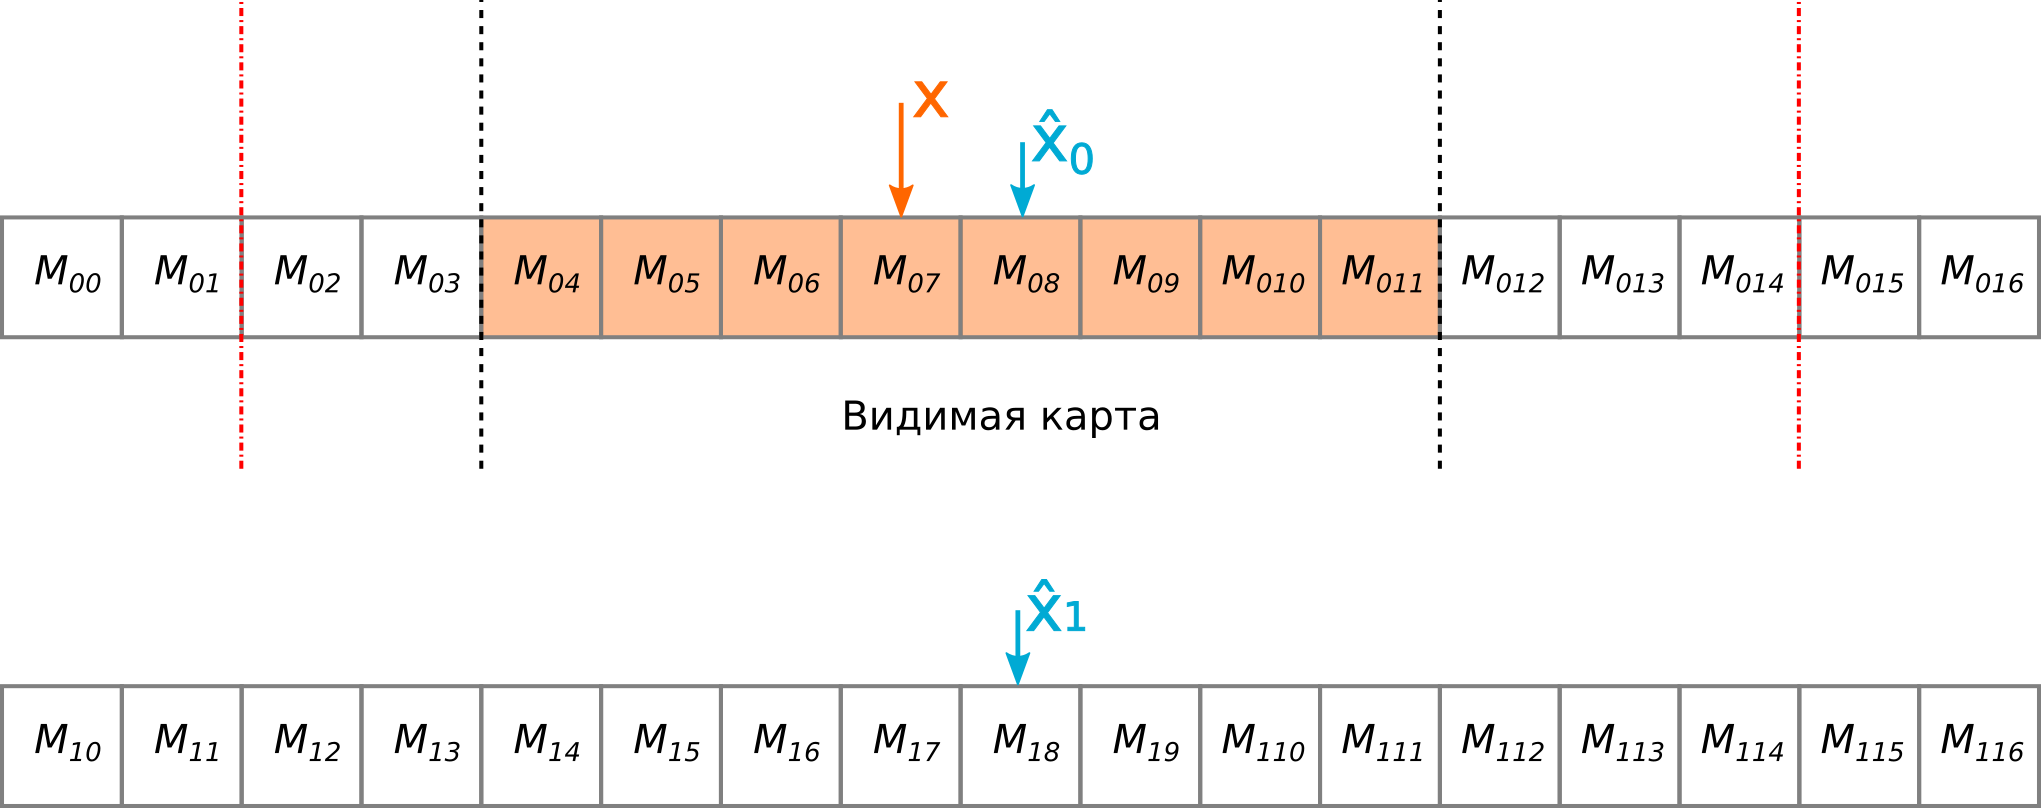
\includegraphics[width=\textwidth]{images/FullyLockFreeOMF.png}
	\caption{Карта с полным обновлением без блокировок.}
	\label{fig:fully_lockfree}
\end{figure}

\textbf{Сдвиг.} Прежде чем приступить к описанию операции, важно сделать следующее замечание: предлагаемая реализация сдвига является неблокирующей относительно добавления фрагмента и получения карты, но в то же время, эта версия не может выполняться одновременно с другими операциями сдвига. 

При сдвиге определяется положение отображаемой карты после сдвига. Если отображаемая часть карты присутствует целиком на одном фрагменте, и в результате сдвига отдаляется от его центра более чем на заданный порог $\Delta_{lim}$ и при этом так же отдаляется и от второго фрагмента (проще говоря, если дальнейшее движение карты в том же направлении приведет к выходу за границы всех фрагментов), то тот фрагмент, на котором сейчас не находится карта, заменяется на новый: все значения клеток (как и ранее это атомарные пары значения логарифма шансов и времени) инициализируются $\{0,0\}$, а его координата меняется таким образом, чтобы при дальнейшем движении в том же направлении отображаемая часть карты <<перешла>> на этот фрагмент (см. рисунок~\ref{fig:fully_lockfree_shift}). В противном случае, как и ранее, положение отображаемой части карты просто обновляется (см. листинг~\ref{alg:fully_lockfree_shift}). В данном алгоритме важно правильно подобрать $\Delta_{lim}$ таким образом, чтобы отображаемая часть карты не могла выйти за границы фрагмента, когда производится замена второго фрагмента (в противном случае это может повлиять на операцию получения карты, выполняемой одновременно со сдвигом).

\begin{figure}[!ht]
	\centering
	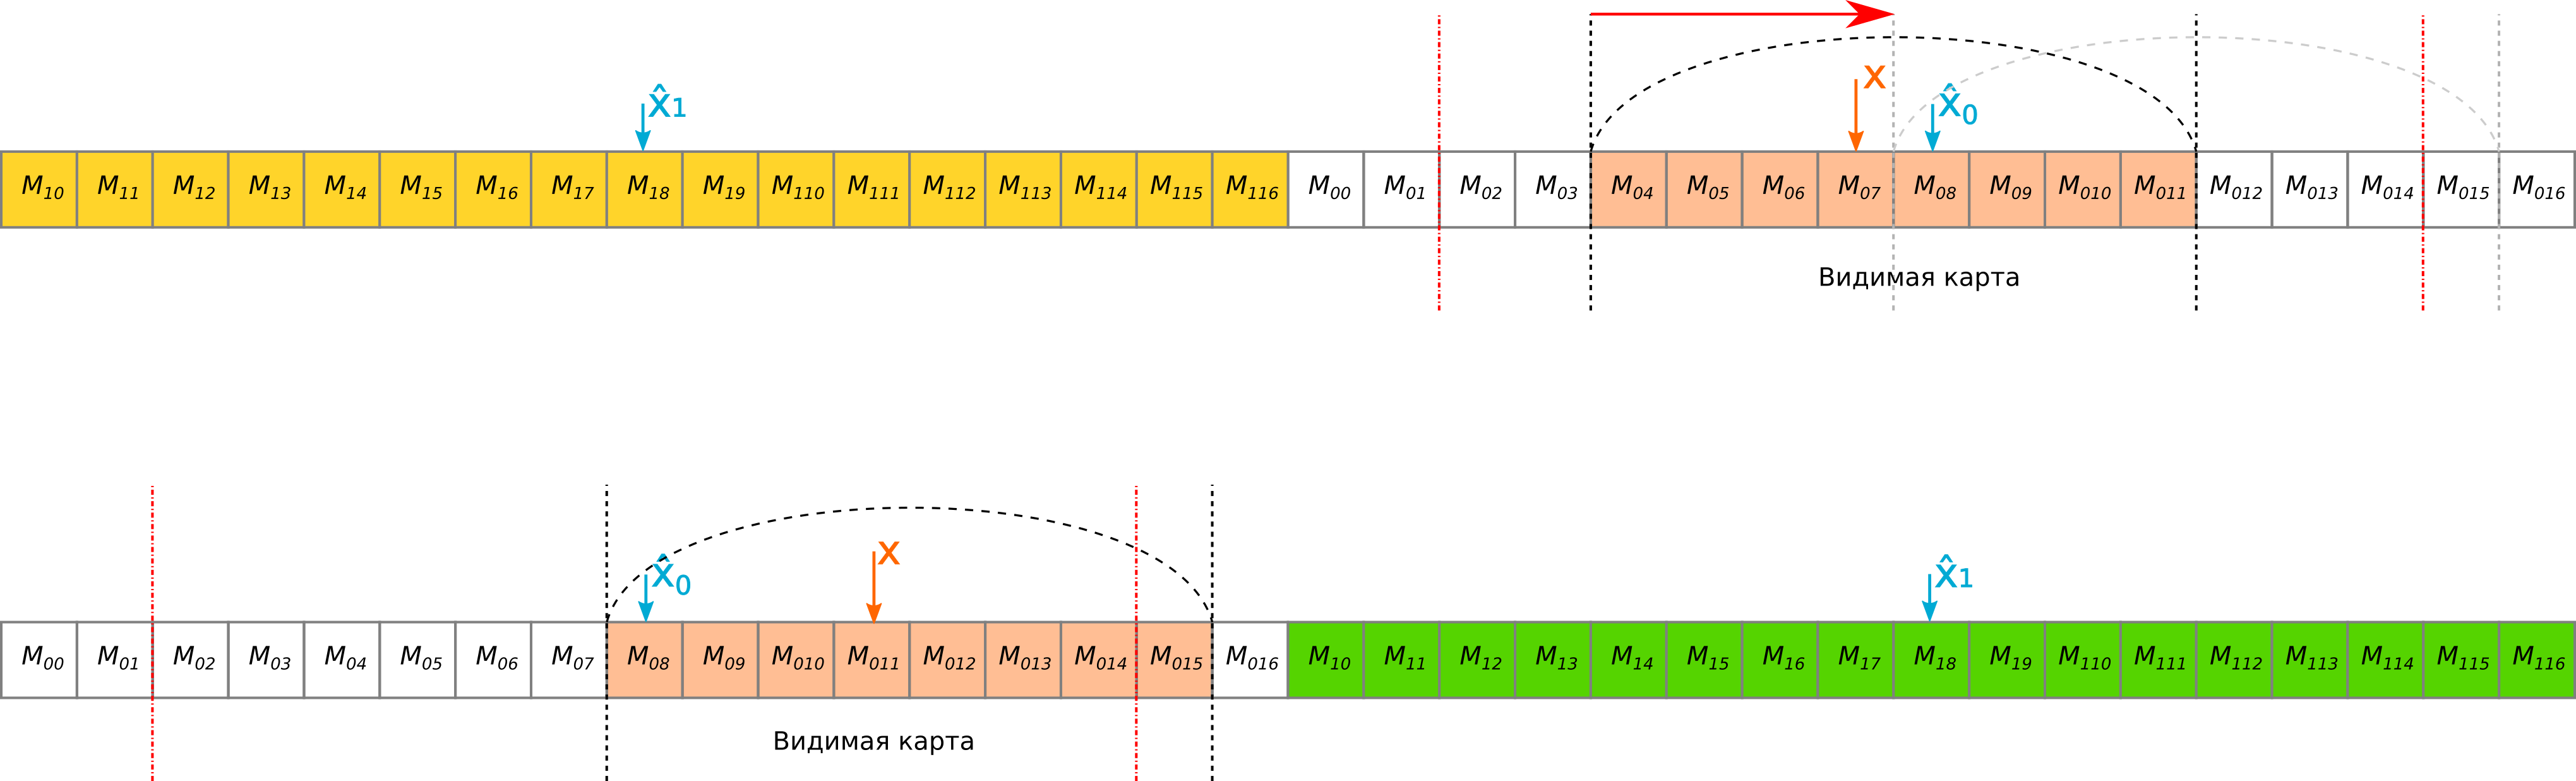
\includegraphics[width=\textwidth]{images/FullyLockFreeOMFShift.png}
	\caption{Сдвиг карты проходимости пространства с полным обновлением без блокировок.}
	\label{fig:fully_lockfree_shift}
\end{figure}

\begin{algorithm}
	\caption{Сдвиг карты (реализация полностью без блокировок): $shift\_map(M, x_{i+1})$.}\label{alg:fully_lockfree_shift}
	\KwIn {$M$ -- карта до сдвига;\\
		$x_{i}$ -- положение $M$ до сдвига;\\
		$x_{i+1}$ -- новое положение карты}
	\KwOut{$M$ после сдвига}
	\If{ $x_{i+1}$ расположен между центрами $M_1$ и $M_2$}{
		\Return{$M$}
	}
	$M_c \gets$ фрагмент ($M_1$ или $M_2$), на котором находится отображаемая карта\;
	$M_o \gets$ оставшийся фрагмент\;
	$\widehat{x} \gets$ центр $M_c$\;
	\If{$\left|\widehat{x} - x_{i+1}\right| > \Delta_{lim}$}{
		$M_{new} \gets$ новый фрагмент размера $\widehat{N}$\;
		\For{ $i \gets 0$ \KwTo $\widehat{N}$}{
			$M_{new}[i] \gets \{0, 0\}$\;
		}
		$M_o \gets M_{new}$\;
	}
	\Return{$M$}
\end{algorithm}

Вычислительная сложность, как и ранее, $\Theta(1)$, в общем случае, когда обновляется только координата отображаемой части локальной карты проходимости пространства. $\Theta(\widehat{N})$, если происходит замена второго фрагмента.

\textbf{Добавление фрагмента} происходит аналогично предыдущим реализациям за исключением следующих моментов:

\begin{enumerate}
	\item В самом начале операции происходит копирование указателей на фрагменты $M_1, M_2$, чтобы гарантировать их сохранение во время выполнения операции (на случай если одновременно с этой операцией выполняется сдвиг, заменяющий один из фрагментов). 
	\item Т.к. операция сдвига не может выполняться одновременно с другими операциями сдвига, в добавлении фрагмента эта операция более не происходит. Вместо этого она либо выполняется в отдельном потоке с определённой частотой (гарантирующей, что отображаемая часть карты всегда содержится на одном или обоих фрагментах карты), либо, например, происходит в операции получения локальной карты проходимости пространства (если гарантируется, что эта операция не выполняется одновременно с такой же)
	\item Операция применяется последовательно к обоим фрагментам карты
\end{enumerate}

Таким образом вычислительная сложность остаётся $O(\min(N_P, N))$. Реальная константа будет незначительно больше, чем в предыдущей реализации из-за атомарного копирования указателей и применения на двух фрагментах (заметим что последнее может быть выполнено одновременно, но асимптотику операции в общем случае это не изменит).

\textbf{Получение карты} также почти не отличается от предыдущей реализации: первым действием операция копирует указатели на фрагменты, чтобы гарантировать сохранность данных во время работы. Вычислительная сложность, как и раньше, $O(N)$.

Сводка вычислительной сложности операций для всех четырёх рассмотренных реализаций приведена в таблице~\ref{tab:complexity_summary}.

\begin{table}[htbp]
	\small
	\centering
	\begin{tabular}{|p{0.27\textwidth}|p{0.14\textwidth}|p{0.28\textwidth}|p{0.13\textwidth}|}
		\hline
		\textbf{Реализация} & \textbf{Сдвиг} & \textbf{Добавление фрагмента} & \textbf{Получение карты} \\
		\hline
		Базовая & $\Theta(N)$ & $O(N + \min(N_P,N))$ & $\Theta(N)$ \\
		\hline
		Расширенная карта & $\Theta(1)$\newline аморт. & $O(\min(N_P,N))$;\newline $O(\widehat{N} + \min(N_P,N))$ при затухании карты & $O(N)$ \\
		\hline
		С разделяемыми блокировками & $\Theta(1)$\newline аморт. & $O(\min(N_P,N))$, допускает одновременное выполнение & $O(N)$ \\
		\hline
		С полным обновлением без блокировок & $\Theta(1)$ & $O(\min(N_P,N))$, допускает одновременное выполнение & $O(N)$ \\
		\hline
	\end{tabular}
	\caption{Вычислительная сложность операций над локальной картой проходимости пространства для базовой реализации и трёх предложенных модификаций. Для операций, допускающих одновременное выполнение несколькими потоками, сложность указана для одного вызова.}
	\label{tab:complexity_summary}
\end{table}

\section{Сравнение задержки обновления локальной карты проходимости пространства}\label{sec:experiments}

Чтобы сравнить представленные модификации между собой, были подготовлены их реализации на C++ и синтетические тесты для измерения времени работы. В рамках этих тестов симулируются следующие сценарии:

\begin{itemize}
	\item Сдвиг карты на $20$ клеток. 
	\item Добавление фрагмента на карту в одном потоке. Размер фрагмента фиксирован и равен 100. Положение фрагмента меняется и берётся из циклической очереди: $-100, -50, -25, -1, 0, 1, 5, 10, 25, 50, 100$. Таким образом моделируются сценарии в которых только часть фрагмента попадает на локальную карту проходимости пространства.
	\item Добавление фрагмента на карту в нескольких потоках. Тот же сценарий, что и в предыдущем пункте, но запускается в нескольких потоках. Протестированы варианты с разным числом потоков: $1, 5, 9, 13$. 
	\item Получение локальной карты проходимости пространства.
	\item Стандартный цикл <<публикации>> локальной карты проходимости пространства: В $8$ потоках производится сдвиг карты на 10 клеток и добавления фрагмента размера $100$, после завершения работы всех потоков, вызывается операция получения карты, имитирующая передачу карты потребителям.
\end{itemize}

Все эксперименты повторялись для <<видимых областей>> разного размера $N$: $10, 16, 32, 64, 128, 256, 512, 1024, 2048, 4000$. Для модификаций принималось значение $\widehat{N} = 2N$ (в случае с последней модификации с полным обновлением без блокировок полный размер карты с учётом неотображаемых областей составил $4N$). Результаты представленных измерений были получены на ПК с процессором AMD Ryzen 5 5600X с 6~ядрами и тактовой частотой 4,6~ГГц, ОЗУ объёмом 32~Гб.

Замеры выполнялись средствами библиотеки Google Benchmark~\cite{googlebenchmark}. Число итераций для каждой точки подбирается библиотекой автоматически, исходя из требуемой длительности замера, и достигает $1,5\cdot10^{6}$. Результатом одного замера служит среднее время итерации. Каждый замер повторялся $10$ раз. На графиках приведены средние значения, коэффициент вариации по повторам не превышает $2,5$~\%. На графиках отложено астрономическое время выполнения, поскольку предметом сравнения является задержка обновления карты. Под коэффициентом линейной аппроксимации далее понимается угловой коэффициент прямой, построенной методом наименьших квадратов по всем десяти размерам карты. Из условий проведения замеров отметим, что масштабирование тактовой частоты процессора не отключалось.

\textbf{Сдвиг карты.} Результаты замеров приведены на рисунке~\ref{fig:bench_shift_put}~а. Исходная реализация растёт линейно, как и было показано при обсуждении её сложности. Остальные реализации имеют в среднем константное время выполнения, поскольку в общем случае требуют лишь обновления координаты $x$, однако их константы различаются. Быстрее всех оказывается реализация с полным обновлением без блокировок, не использующая мьютексы для создания критических секций; далее следует расширенная карта, использующая стандартный std::mutex; худшее время среди модификаций показывает карта с разделяемыми блокировками, поскольку манипуляции с std::shared\_mutex вычислительно более интенсивны. Отметим также, что на малых размерах карты исходная реализация эффективнее всех модификаций.

\textbf{Добавление фрагмента в одном потоке.} Результаты приведены на рисунке~\ref{fig:bench_shift_put}~б. Как и в предыдущем сценарии, исходная реализация имеет линейную сложность; ту же сложность показывает и расширенная карта, что объясняется необходимостью приводить все клетки массива к одному моменту времени. Этим же объясняется и большее время расширенной карты в сравнении с исходной: ей требуется обновить большее число клеток. Оставшиеся две модификации с ростом размера карты выходят на постоянное число операций, так как обновляют не всю карту, а только клетки, пересекающиеся с фрагментом. При этом реализация без блокировок уступает реализации с разделяемыми блокировками: вероятная причина -- атомарное копирование указателей на фрагменты, обращение к элементам через указатель и повторение операции на двух массивах; последние два фактора снижают локальность данных и увеличивают число промахов кэша.

\begin{figure}[!ht]
	\centerfloat{
		\subcaptionbox{Сдвиг карты.\label{fig:bench_move}}{
			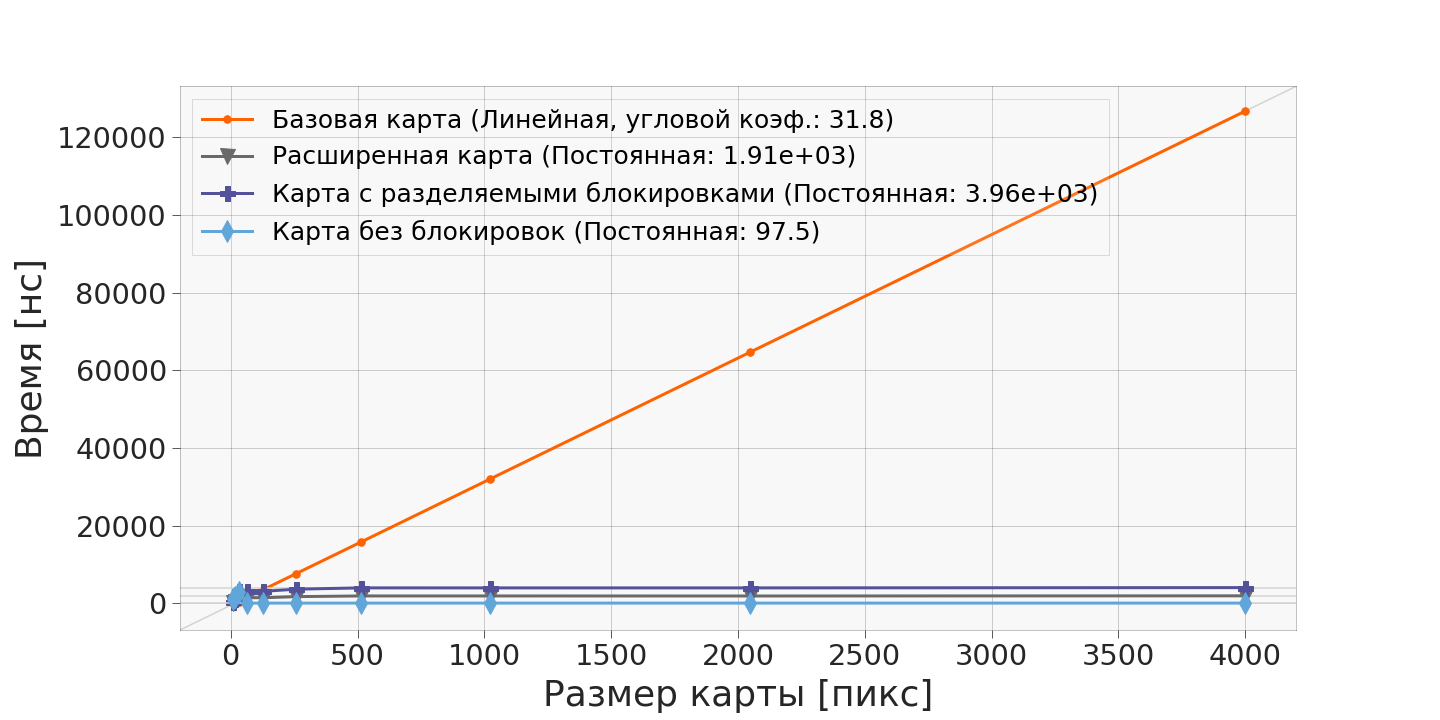
\includegraphics[width=0.82\linewidth]{images/_MoveMap_it4.png}}\\
		\subcaptionbox{Добавление фрагмента в одном потоке.\label{fig:bench_put_single_thread}}{
			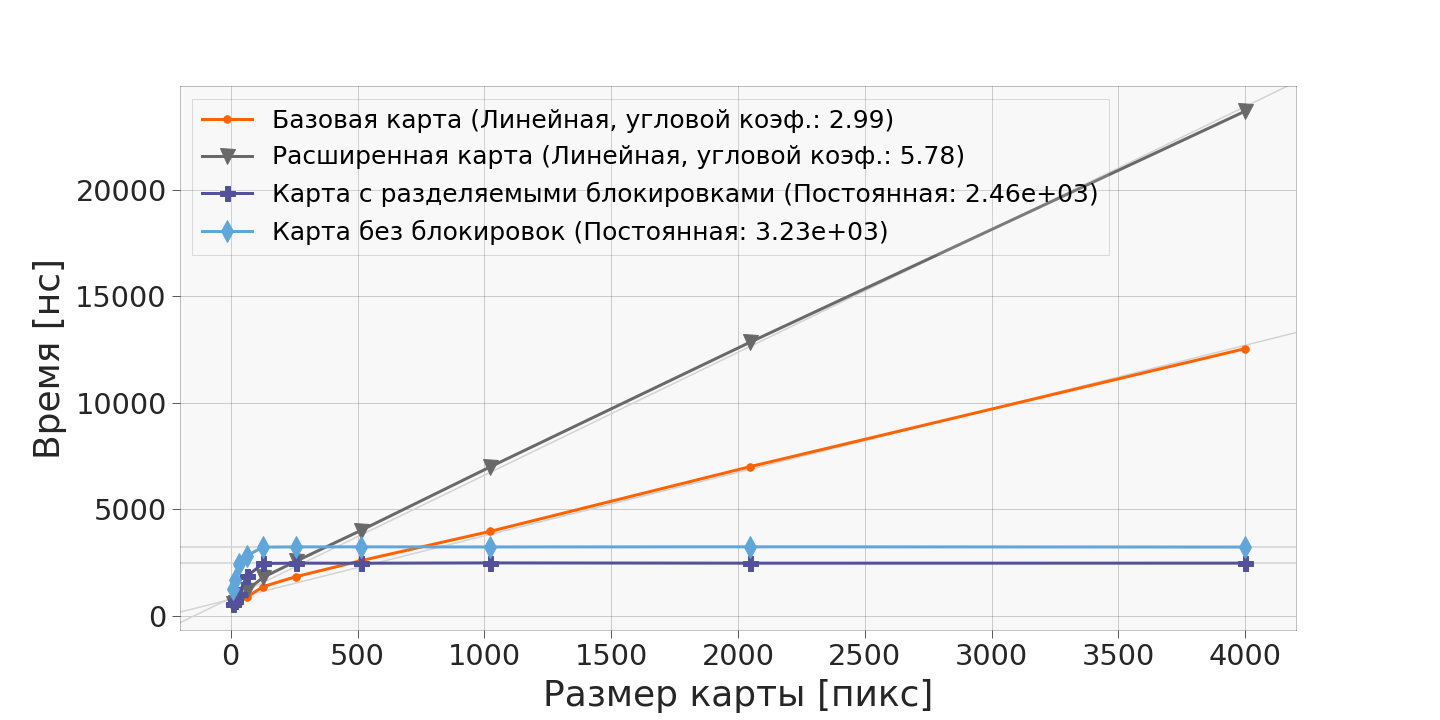
\includegraphics[width=0.82\linewidth]{images/_PutPatch_it4.png}}\\
	}
	\caption{Графики зависимости времени выполнения операций над локальной картой проходимости пространства от размера карты.}\label{fig:bench_shift_put}
\end{figure}

\textbf{Добавление фрагмента в нескольких потоках.} Результаты замеров приведены на рисунке~\ref{fig:bench_put_multi}. Здесь применимы рассуждения предыдущего сценария; сценарий с одним потоком отличается от предыдущего замера только наличием обвязки для запуска в пуле потоков. Можно отметить, что с ростом числа потоков уменьшается размер карты, начиная с которого модификации с частичным или полным отказом от блокировок становятся вычислительно эффективнее исходной реализации.

\begin{figure}[!ht]
	\centering
	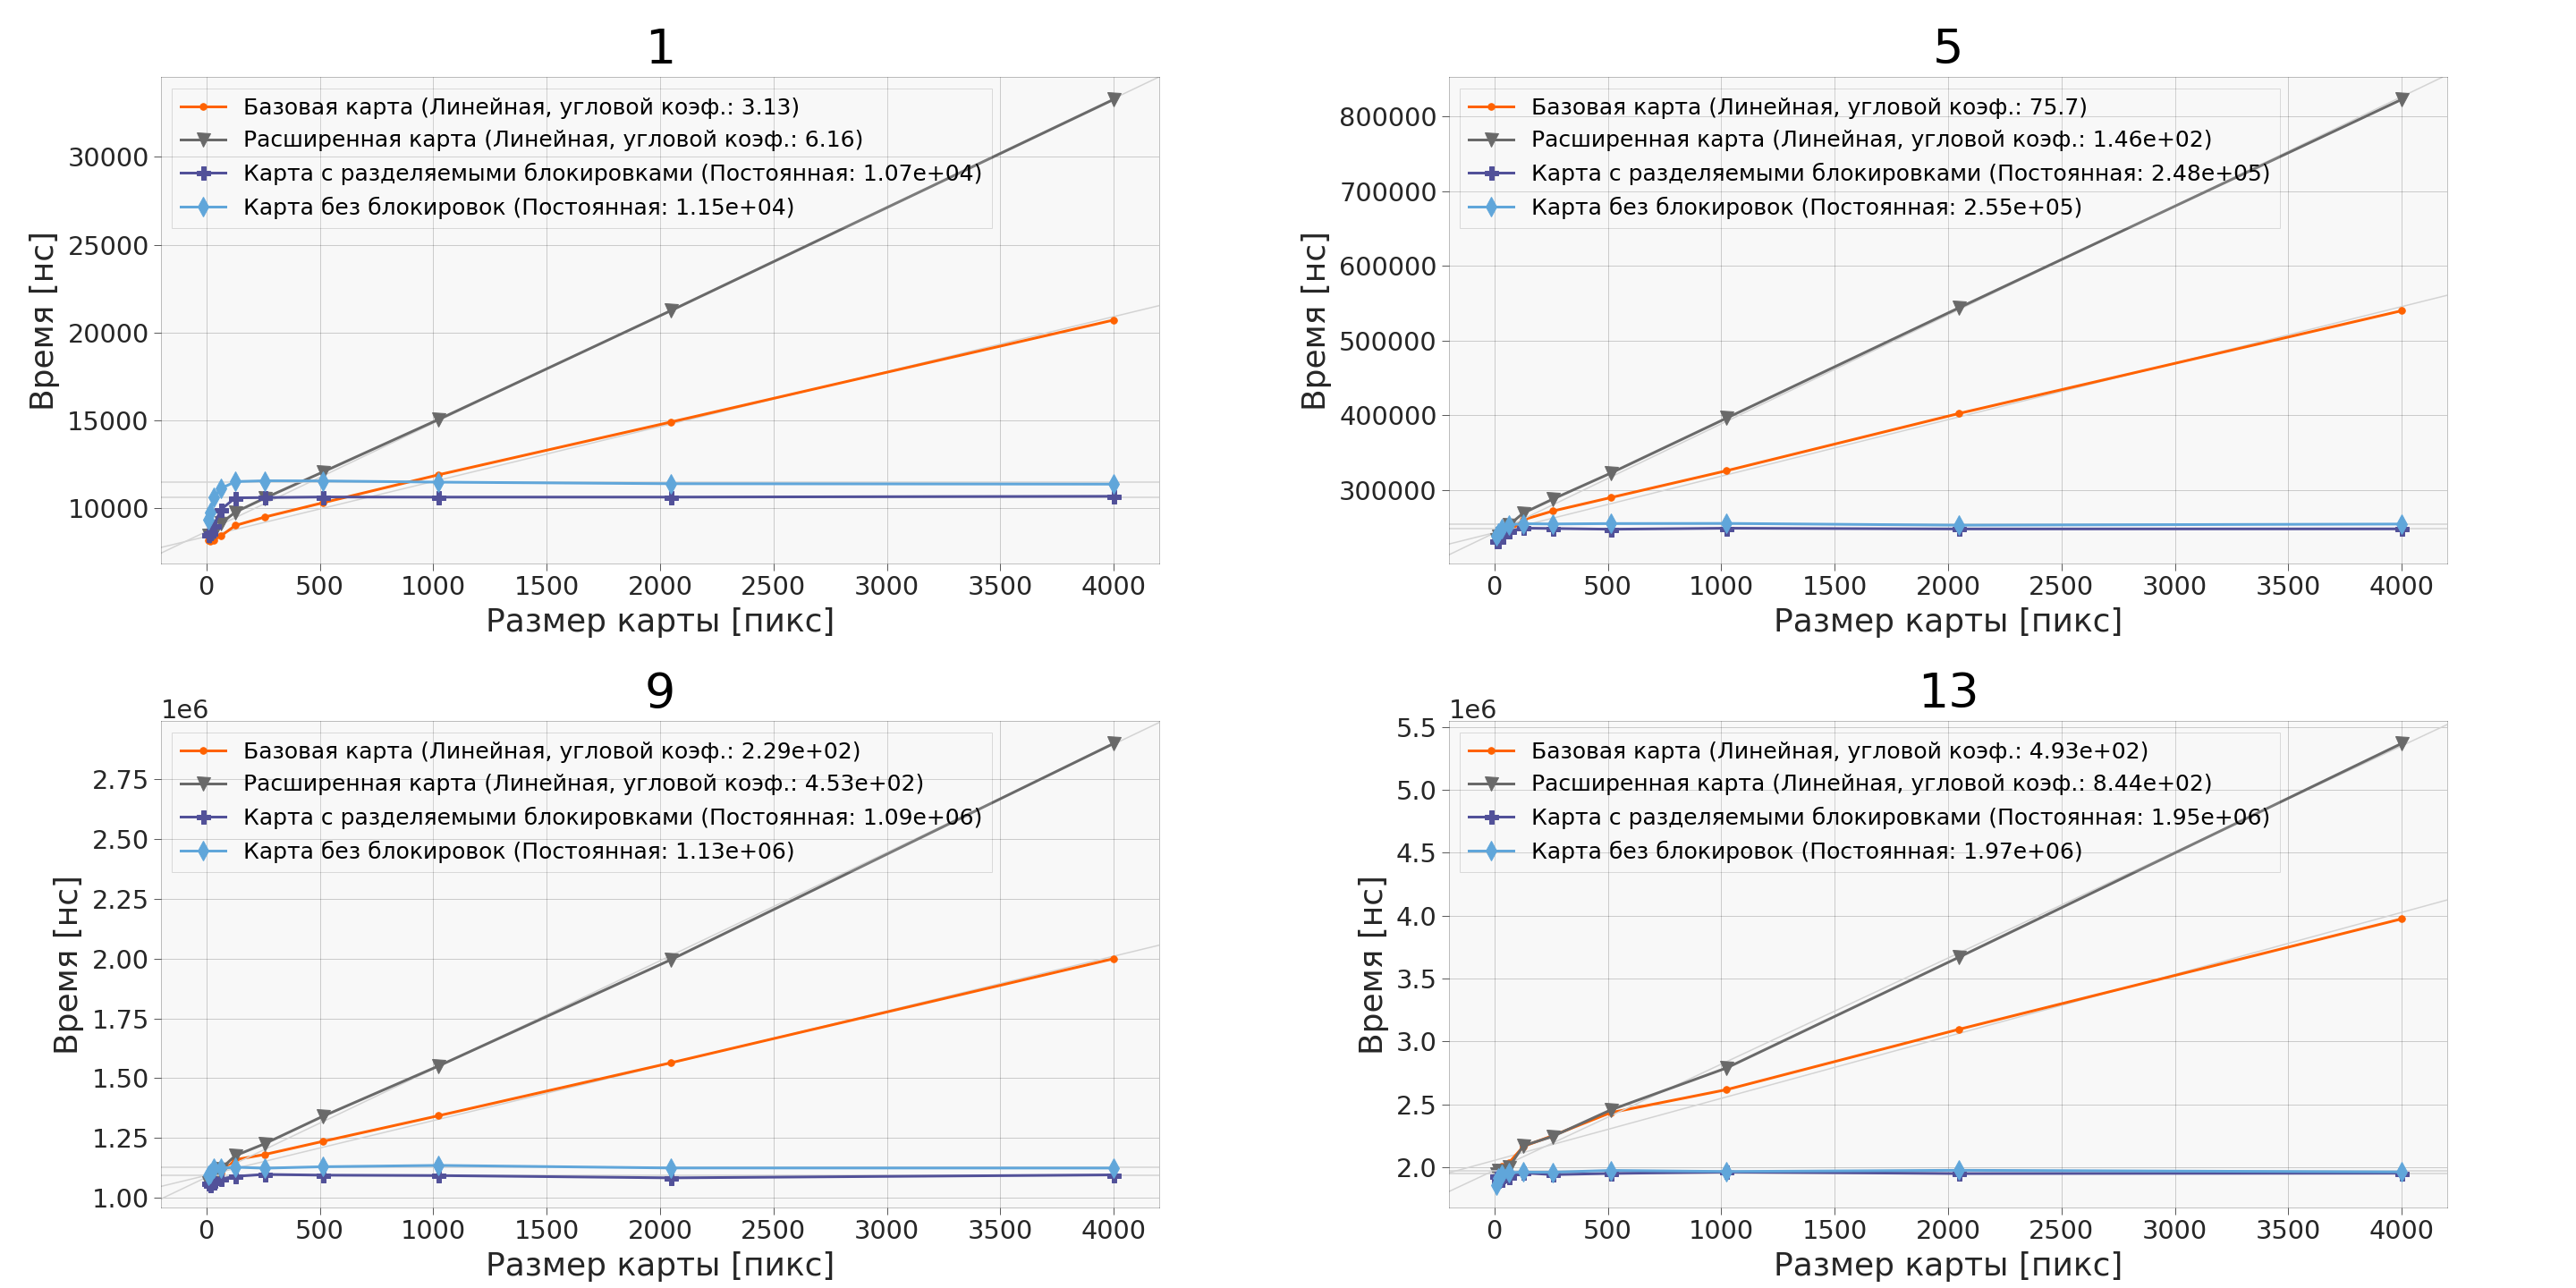
\includegraphics[width=\linewidth]{images/ParallelPutPatch.png}
	\caption{Графики зависимости времени добавления фрагмента на карту от размера карты при $1$, $5$, $9$ и $13$ потоках.}
	\label{fig:bench_put_multi}
\end{figure}

\textbf{Получение карты.} Результаты приведены на рисунке~\ref{fig:bench_get_iter}~а и заметно отличаются от предыдущих сценариев. Время получения карты у исходной реализации и у расширенной карты с ростом размера карты возрастает настолько медленно, что на фоне реализаций с частичным или полным отказом от блокировок кажется константным, хотя и остаётся линейным. У последних же из-за необходимости атомарно считывать значения клеток и приводить их к общему моменту времени время работы увеличивается значительно быстрее.

\textbf{Стандартный цикл <<публикации>> карты.} Это наиболее показательный сценарий: он определяет, какая реализация окажется лучше в реальном режиме работы. Результаты приведены на рисунке~\ref{fig:bench_get_iter}~б. Все реализации имеют линейную вычислительную сложность относительно размера карты, и все предложенные модификации превосходят исходную реализацию, причём каждая следующая модификация показывает себя лучше предыдущей -- по крайней мере по мере увеличения размера карты. Лучшую производительность показала реализация с полным обновлением без блокировок: экспериментально установленный для неё коэффициент линейной аппроксимации зависимости времени одной итерации от размера карты в $13,5$ раза меньше, чем у исходной реализации. Далее следует модификация с разделяемыми блокировками (в $10,3$ раза быстрее исходной реализации). Наконец, расширенная карта при всей своей тривиальности дала прирост производительности в $6,2$ раза.

\begin{figure}[!ht]
	\centerfloat{
		\subcaptionbox{Получение карты. График базовой реализации практически совпадает с расширенной картой и на таком масштабе от неё неотличим.\label{fig:bench_get}}{
			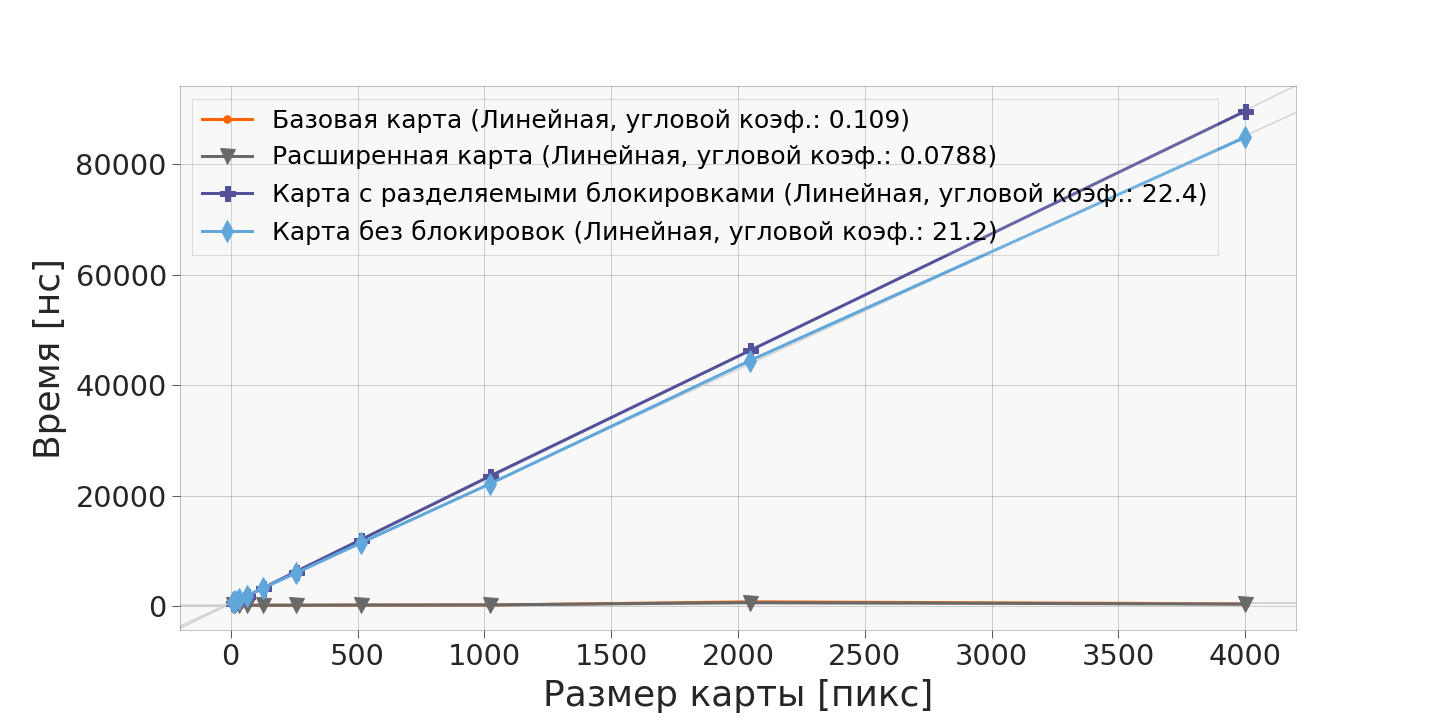
\includegraphics[width=0.82\linewidth]{images/_GetMap_it4.png}}\\
		\subcaptionbox{Одна итерация <<публикации>> карты.\label{fig:bench_iter}}{
			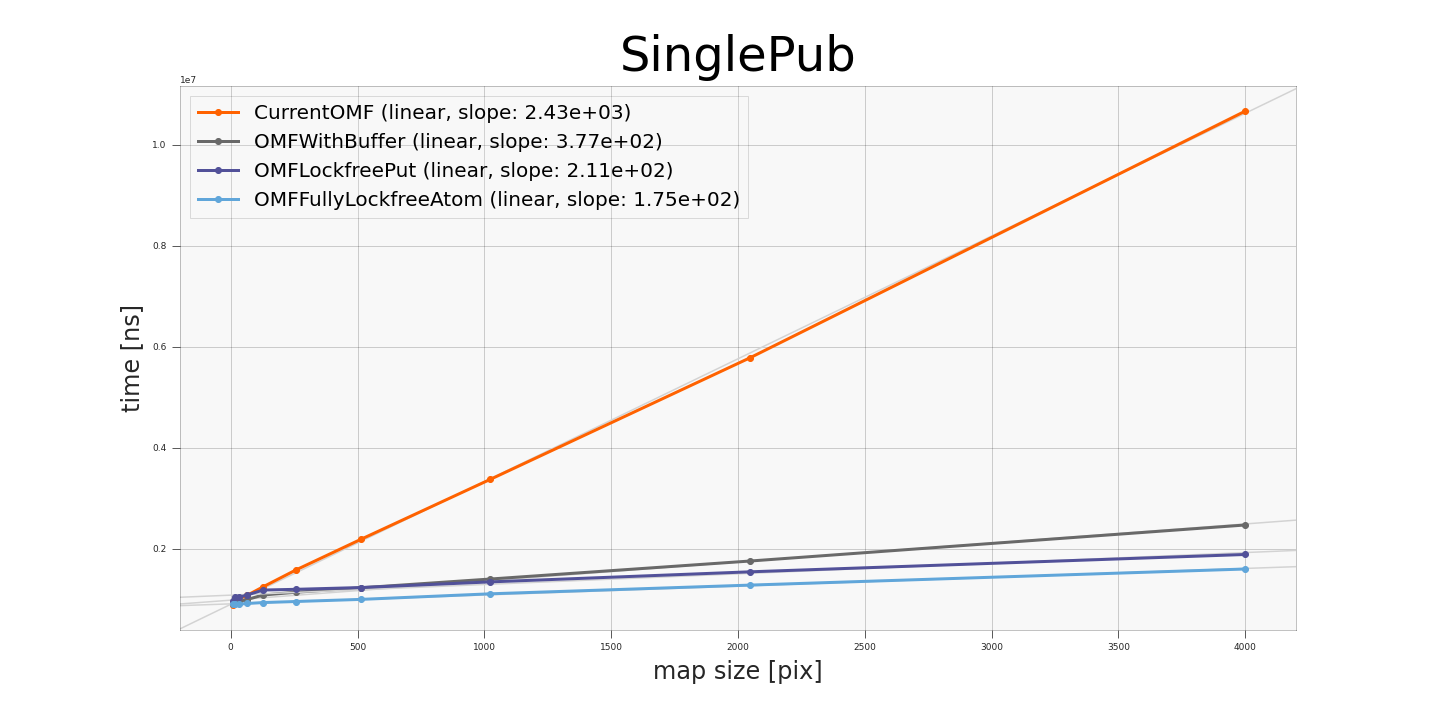
\includegraphics[width=0.82\linewidth]{images/_SinglePub_it4.png}}\\
	}
	\caption{Графики зависимости времени получения карты и времени одной итерации <<публикации>> карты от размера карты.}\label{fig:bench_get_iter}
\end{figure}


\section{Реализация финальной модификации для двумерной карты проходимости пространства}\label{sec:2D_implementation}

Показав работоспособность и лучшую производительность модификации локальной карты проходимости пространства с полным обновлением без блокировок в одномерном случае, представим её расширение для двумерного случая. Как и ранее, полная карта окружения разбивается на несколько, теперь уже двумерных, массивов, состоящих из уже описанных ранее атомарных пар логарифма шансов и времени. Для движения в плоскости потребуется $9$ массивов (рисунок~\ref{fig:lockfree_2d}). Если видимая область карты пересекает границы, отмеченные штрих-пунктирной линией, создаются новые массивы и заменяют часть предыдущих таким образом, чтобы текущий массив, в котором находится видимая область карты, стал центральным. Важно отметить, что отступ этих линий от краёв массива должен быть подобран так, чтобы за одну итерацию сдвига, видимая область не могла преодолеть расстояние между линией и границей массива. В противном случае если параллельно будет происходить получение карты, то массив, в который <<переходит>> видимая область, может быть ещё не создан, что приведёт к ошибке выполнения.

\begin{figure}[htbp]
	\centering
	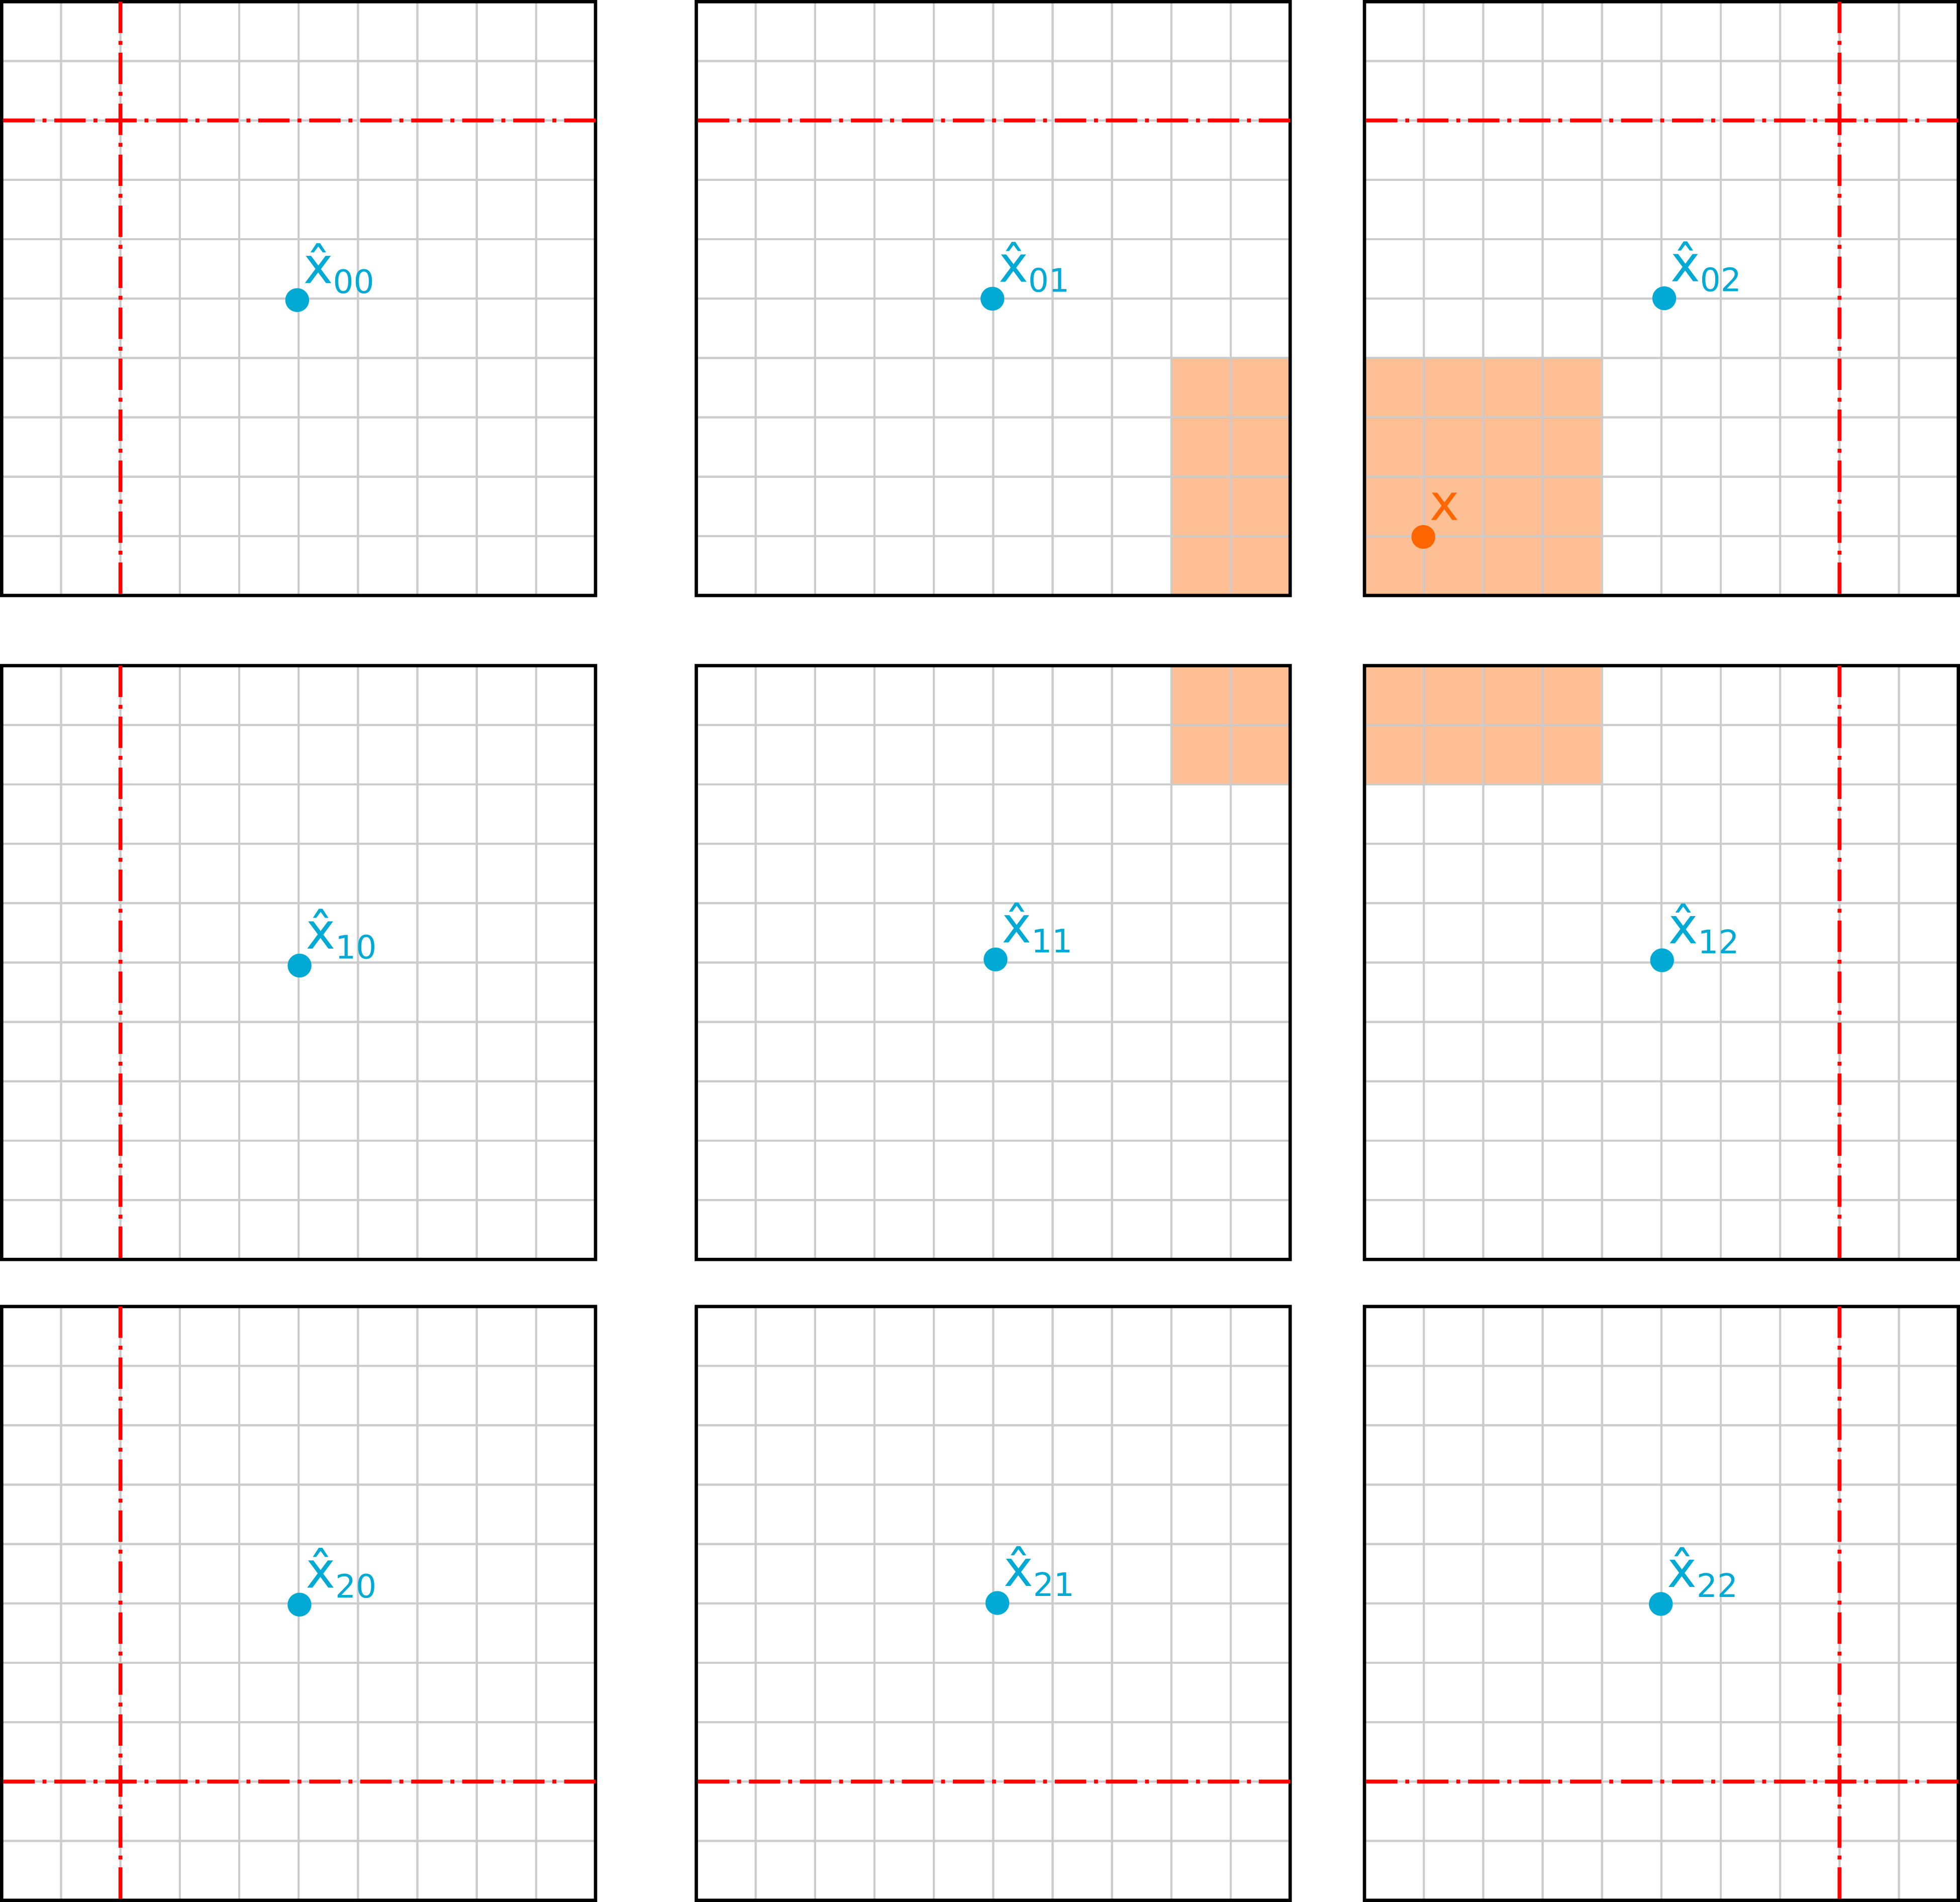
\includegraphics[width=0.6\linewidth]{images/Lockfree2D.png}
	\caption{Двумерная реализация локальной карты проходимости пространства с полным обновлением без блокировок.}
	\label{fig:lockfree_2d}
\end{figure}

Плата за такую реализацию двояка. Во-первых, она значительно увеличивает объём памяти, требуемой для хранения структуры данных. Во-вторых, как и в одномерном случае, операции получения карты и добавления фрагмента применяются ко всем $9$ массивам, что увеличивает коэффициент линейной аппроксимации времени их выполнения. Определение условий, при которых такая реализация вычислительно эффективнее исходной, требует дополнительных экспериментов: результат зависит от средней скорости движения БТС, среднего размера добавляемых фрагментов, числа источников данных и частоты их работы, а также от масштаба локальной карты проходимости пространства. Тем самым установленный в разделе~\ref{sec:experiments} выигрыш относится к модельной одномерной задаче; перенос двумерной реализации на бортовой вычислитель БТС и измерение задержки обновления карты в тех же условиях, в которых выполнено профилирование раздела~\cref{sec:ch4/perf}, составляют предмет дальнейшей работы.

\section{Заключение к главе~\ref{ch:ch4}}

В главе получены следующие результаты:

\begin{enumerate}
	\item выполнено профилирование программного комплекса, представленного в главе~\cref{ch:ch3}, при одном и восьми одновременно подключённых источниках данных. Время обновления карты составило $3,03$ и $22,78$~мс соответственно: комплекс укладывается в ограничение $100$~мс, обеспечивающее работу при частоте регистрации данных $10$~Гц	. Вместе с тем рост задержки более чем в семь раз при переходе от одного источника к восьми показывает, что последовательное добавление фрагментов ограничивает дальнейшее наращивание их числа;
	\item предложены три последовательные модификации алгоритма построения локальной карты проходимости пространства, направленные на снижение вычислительной сложности производимых операций;
	\item произведена оценка вычислительной сложности предложенных алгоритмов;
	\item алгоритмы реализованы в виде программного кода на языке C++ и протестированы для упрощённого сценария одномерной карты проходимости пространства. Полученные при тестировании результаты:
	\begin{enumerate}
	\item теоретические оценки сложности алгоритмов подтверждены экспериментально;
	\item лучшую скорость добавления фрагмента на карту в одном и нескольких потоках показала вторая модификация -- карта с разделяемыми блокировками;
	\item лучшую скорость получения карты проходимости показала оригинальная реализация карты;
	\item лучшую скорость сдвига карты показала последняя модификация -- карта проходимости пространства с полным обновлением без блокировок;
	\item в симуляции одного цикла публикации карты проходимости пространства лучшая производительность продемонстрирована последней модификацией: коэффициент линейной аппроксимации зависимости времени итерации от размера карты уменьшился в $13,5$ раза относительно базовой реализации;
    \end{enumerate}
	\item предложено расширение последней модификации карты проходимости пространства для двумерного пространства.
\end{enumerate}

Отметим, что достигнутый выигрыш представляет собой размен, а не улучшение по всем показателям сразу. Он получен на составном цикле публикации карты и оплачен замедлением операции получения карты: коэффициент линейной аппроксимации для неё возрастает с $0,109$ до $21,2$~нс на элемент, то есть почти на два порядка. К этому добавляется рост потребления памяти -- в одномерном случае вчетверо относительно отображаемой области. Выигрыш достигается за счёт того, что в цикле публикации операции добавления фрагмента и сдвига карты выполняются многократно чаще операции её получения.

Перечисленные основные результаты и другие авторские материалы главы опубликованы в работе~\cite{чеканов2026многопоточные}.

\clearpage